\documentclass[fin1, tisk]{fmfdelo}

%%%%%%%%%%%%%%%%%%%%%%%%%%%%%%%%%%%%%%%%%%%%%%%%%%%%%%%%%%%%%%%%%%%%%%%%%%%%%%%
% METAPODATKI
%%%%%%%%%%%%%%%%%%%%%%%%%%%%%%%%%%%%%%%%%%%%%%%%%%%%%%%%%%%%%%%%%%%%%%%%%%%%%%%

\avtor{Neža Kržan}
\naslov{Statistika v kazenskem pravu}
\title{Criminal justice statistics}
\mentor{izr. prof. dr. Jaka Smrekar}
\letnica{2023}

\povzetek{
Diplomsko delo opisuje uporabo verjetnosti in statistike v kazenskem pravu. Statistične metode so temelj kazenskega pravosodja in kriminologije, 
pa ne le za raziskave, pri katerih so podlaga statistični podati in analize, ampak tudi za vrednotenje hipotez in dokazov sodnega procesa. Čedalje 
pogosteje je, da velik del zaključka sodnega procesa temelji na verjetnostnem izračunu vpliva dokazov na začetno in vmesne hipoteze. Koncept verjetnosti 
temelji na primerjavi verjetnosti dokazov na podlagi dveh konkurenčnih predlogov, in sicer predloga tožilstva in predloga obrambe in je ključen pri 
ocenjevanju dokazov, saj nam zagotovi objektivno oceno njihovega vpliva na verjetnost določene domneve oziroma hipoteze. Pri presoji dokazov se 
uporablja različne metode in nekatere izmed njih sem opisala v diplomskem delu. \\
Najpogosteje uporabljena metoda in tudi ena izmed najbolj razvitih temelji na Bayesovi statistiki. Bayesova statistika je statistična veja, ki nam s 
pomočjo matematičnih pristopov omogoča posodabljanje predhodnih oziroma apriornih verjetnosti dokazov v posteriorno verjetnost. Težave se pojavijo 
pri določitvi predhodnih verjetnosti, saj je deljeno mnenje kdo naj določi te verjetnosti in na kakšen način. Različne metode za določitev lahko 
dajejo različne rezultate, kar pa je problematično, saj celotna Bayesova teorija temelji ravno na teh začetnih izračunih. Zaradi verjetnostne 
oblika Bayesovega izreka, za merilo vrednosti dokazov uporabljamo razmerje verjetnosti.\\
Ker pa je statistika v kazenskem pravu še v razvoju in je znanje ter razumevanje verjetnosti precej omejeno pri odvetnikih, sodnikih in 
poroti, se pojavlja mnogo zmot. Najbolj znana primera takih zmot sta Tožilčeva zmota, ki je dobro znan statistični problem, druga večja, ki 
pa izhaja iz prve, pa je Zmota obrambnega odvetnika in ker zmoti največkrat 
nista prepoznani, je posledica lahko tudi napačen zaključek sodnega procesa. Tožilčeva zmota temelji na zamenjavi dveh različnih pogojnih 
verjetnosti, ki imata zelo različni vrednosti. Pri Zmoti obrambnega odvetnika pa dokaze obdolženca, ki se ujemajo z dokazi kaznivega 
dejanja štejejo za nepomembne. Večina ostalih zmot prav tako izhaja iz napačnega razumevanja pogojne verjetnosti. \\
Ker so zmote velik problem, opišem tudi nekatere ustrezne pristope za izogib zmotam, pri čemer je po mojem mnenju najbolj učinkovit 
pristop uporaba Bayesovih omrežij, ker nam pomagajo določiti ustrezne verjetnostne formule v grafičnih modelih, ne da bi prikazali njihovo 
popolno algebrsko obliko. Bistveno izboljšajo vrednotenje verjetnostnih razmerij, ki se uporabljajo za ocenjevanje dokazov in omogočajo 
kompleksnejše analize. Za njihovo izdelavo je potreben dosleden okvir, sicer lahko pridemo do različnih rezultatov. Ker pa izračun verjetnosti 
hipotez in dokazov ponovno temelji na Bayesovi teoriji, se pomanjkljivost Bayesove statistike prenese tudi na Bayesova omrežja.
} 

\abstract{In this Bachelor’s thesis we describe the use of probability and statistics in criminal justice. Statistical methods are the foundation of criminal justice and criminology, not only for research based on statistical data and analysis, but also for evaluating hypotheses and evidence in the judicial process. Increasingly, a significant portion of the conclusion of legal proceedings is based on probabilistic calculations of the impact of evidence on initial and intermediate hypotheses. The concept of probability relies on comparing the probability of evidence based on two competing propositions, namely the prosecution's proposition and the defense's proposition, and is crucial in assessing evidence as it provides an objective evaluation of their impact on the probability of a particular assumption or hypothesis. In this Bachelor’s thesis we also describe methods that are used in the assessment of evidence.\\
The most commonly used method, and also one of the most developed, is based on Bayesian statistics. Bayesian statistics is a statistical branch that employs mathematical approaches to update prior probabilities of evidence into posterior probabilities. Challenges arise in determining prior probabilities, as there is a divided opinion on who should establish these probabilities and in what manner. Different methods of determination can yield different results, which is problematic since the entire Bayesian theory relies on these initial calculations. Due to the probabilistic nature of the Bayesian theorem, the measure of the evidential value uses the likelihood ratio.\\
As statistics in criminal law is still evolving and the knowledge and understanding of probability are quite limited among lawyers, judges, and juries, numerous misconceptions arise. The most well-known examples of such misconceptions are the Prosecutor's Fallacy, which is a well-known statistical problem, and a more significant fallacy stemming from it, known as the Defense Attorney's Fallacy. Because these fallacies often go unrecognized, their consequence can be an incorrect conclusion in the judicial process. The Prosecutor's Fallacy is based on the confusion of two different conditional probabilities with vastly different values. In the Defense Attorney's Fallacy, evidence presented by the accused that matches evidence of the criminal act is considered insignificant. Most other fallacies also arise from a misunderstanding of conditional probability. \\
Because fallacies are a significant issue, I also describe some appropriate approaches to avoid them. In my opinion, the most effective approach is the use of Bayesian networks, as they help us determine appropriate probability formulas within graphical models without displaying their complete algebraic form. They significantly enhance the evaluation of likelihood ratios used for evidence assessment and enable more complex analyses. Constructing them requires a consistent framework, as inconsistent approaches can yield different results. However, since the computation of hypotheses and evidence probabilities once again relies on Bayesian theory, the shortcomings of Bayesian statistics are also transferred to Bayesian networks.
}

\klasifikacija{62P99, 62C10, 60A99}
\kljucnebesede{bayesova statistika\sep predhodna verjetnost\sep posteriorna verjetnost\sep razmerje verjetnosti\sep frekvence\sep tožilčeva zmota\sep bayesova omrežja}
\keywords{bayesian statistics\sep apriori probability\sep posterior probability\sep likelihood ratio\sep frequencies\sep prosecutor's fallacy\sep bayesian networks}

\slovar{
 \geslo{apriori probability}{predhodna verjetnost}
 \geslo{posterior probability}{posteriorna verjetnost}
 \geslo{likelihood ratio}{razmerje verjetnosti}
 \geslo{fallacy}{zmota}
 \geslo{prosecutor's fallacy}{tožilčeva zmota}
 \geslo{defense attorney's fallacy}{zmota obrambnega odvetnika}
 \geslo{network}{omrežje}
}

\literatura{literatura.bib}

%%%%%%%%%%%%%%%%%%%%%%%%%%%%%%%%%%%%%%%%%%%%%%%%%%%%%%%%%%%%%%%%%%%%%%%%%%%%%%%
% DODATNE DEFINICIJE
%%%%%%%%%%%%%%%%%%%%%%%%%%%%%%%%%%%%%%%%%%%%%%%%%%%%%%%%%%%%%%%%%%%%%%%%%%%%%%%
\usepackage[T1]{fontenc}
\usepackage[utf8]{inputenc}
\usepackage{amsmath,amssymb,amsfonts}
\usepackage{url}
\usepackage[normalem]{ulem}
\usepackage[dvipsnames,usenames]{color}
\usepackage{graphicx}
\usepackage{lipsum}
\usepackage[slovene]{babel}
\usepackage{float}
\usepackage{breakurl} % Break URLs over multiple lines
\usepackage{hyperref} % Link bibliography links (avoid long links for clarity)
\usepackage{etoolbox}

\restylefloat{table}

\theoremstyle{definition} 
\theoremstyle{trditev} 
\theoremstyle{izrek}


%%%%%%%%%%%%%%%%%%%%%%%%%%%%%%%%%%%%%%%%%%%%%%%%%%%%%%%%%%%%%%%%%%%%%%%%%%%%%%%%%%%%%%%%%%%%%%%%%%%%%%%%%%%%%%%%%%%%%%%%%%%%%%%%%%%%%%%%%%%%%%
% ZAČETEK VSEBINE
%%%%%%%%%%%%%%%%%%%%%%%%%%%%%%%%%%%%%%%%%%%%%%%%%%%%%%%%%%%%%%%%%%%%%%%%%%%%%%%%%%%%%%%%%%%%%%%%%%%%%%%%%%%%%%%%%%%%%%%%%%%%%%%%%%%%%%%%%%%%%%
\begin{document}

\nocite{collins,byers,aitkena,hoff,aitkenb,aitkenc,aitkend,bello,berger,conklin,dahlman,fentona,fentonb,finkelstein,gastwirth,giannini,glover,iliinski,maarcot,macedo,maddan,matthews,orban,schumana,schumanb,scurich,balaba,blankenship,skorupski,balding,bidermann,tarling}

\section{Uvod}
Statistične metode za vrednotenje dokazov v sodnih procesih so se začele uporabljati že v letih prejšnjega stoletja. Iz znanih teorij verjetnosti in
statistike so se razvile metode za čim boljše ocenjevanje in vrednotenje dokazov na podlagi začetnih hipotez. Zaradi pomanjkanja znanja teorije
verjetnosti so se hitro začele pojavljati zmote statističnih analiz dokazov. Ker do večina zmot pride pri napačnem razumevanju končnega rezultata
statistične analize, so danes v razvoju novi načini za predstavitev le teh. Poleg tega se problema zavedajo tudi pravne fakultete, ki v ta namen v svoje učne
programe že vključujejo teorijo statistike in verjetnosti. Težava pa ni le pri razumevanju končnega poročila, ampak tudi pri analizi in vrednotenju
dokazov. Statistični znanstveniki se srečujejo s problemi metod vrednotenja in upoštevanjem pravnih zakonov in teorije. V diplomskem delu poskušam
čim bolje predstaviti nekatere metode za vrednotenje dokazov, njihove pomanjkljivosti in prednosti. Poleg tega pa poskušam najti način čim hitrejše
analize dokazov in hkrati tudi najboljši prikaz končnega poročila analize poroti, sodnikom in odvetnikom v skladu s pravnimi pravili.\\\\
Diplomsko delo je razdeljeno v več razdelkov. Najprej so opredeljeni osnovni koncepti statistike v kazenskem pravu in predstavljen je 
razsikovalni proces za preučevanje problemov kriminologije. Nato sledi opis vrednotenja dokazov in konept verjetnosti v kazenskem 
pravu. V glavnem delu diplomske naloge predstavim metode vrednotenja dokazov in se osredotočim na podroben opis Bayesove statistike 
v kazenskem pravu in njene uporabe pri ugotavljanju, ali je obtoženec vir sledi DNK-ja s kraja zločina. Ker je Bayesova statistika 
na nek način tehtanje dokazov opredelim tudi razmerje verjetnosti, ki je potrebno za določitev vrednosti dokaza oziroma dokazov. Za 
primerno predstavo prednosti in slabosti Bayesove teorije v kazenskem pravu, opišem še metodo frekvenc in njeno uporabo pri DNK dokazih 
ter metodo verjetnosti naključnega ujemanja. V zadnjem delu sledi predstavitev zmot, ki nastanejo zaradi napačnega razumevanja verjetnosti 
in možni pristopi za odpravo oziroma izogib le teh. Opis statistike v kazenskem pravu podkrepim s predstavitvijo kazenskega primera medicinske 
sestre Lucie De Berg, v katerem prikažem glavne težave s katerimi se srečujejo statistični analitiki. Poleg tega so tudi vmesni pojmi, 
poleg teoretične opredelitve, podprti s primerljivimi primeri za lažjo predstavo.\\\\
Cilj dela diplomskega seminarja je spoznavanje uporabnosti statistike in verjetnosti na manj znanem področju kot je kazensko pravo. Ker je koncept 
verjetnosti v kazenskem pravu še v razvoju me zanimajo predvsem napake in pomanjkljivosti. Želela bi ugotoviti katere metode vrednotenja 
dokazov in ocenjevanja verjetnosti hipotez so najboljše in kako se najlažje izogniti Tožilčevi zmoti in zmoti Obrambnega odvetnika. Namen 
naloge ni predstaviti vseh metod, ki jih uporabljajo za vrednotenje dokazov, ker se ravno zaradi razvoja vede, to hitro posodablja. Zanimajo pa 
me tudi možne napake in težave, ki se zgodijo pred predstavitvijo rezultatov statističnih analiz na sodišču. Osredotočila se bom 
predvsem na evropsko kazensko pravo in evropske kazenske primere, ter svoje zaključke napisala na podlagi teh.

%%%%%%%%%%%%%%%%%%%%%%%%%%%%%%%%%%%%%%%%%%%%%%%%%%%%%%%%%%%%%%%%%%%%%%%%%%%%%%%%%%%%%%%%%%%%%%%%%%%%%%%%%%%%%%%%%%%%%%%%%%%%%%%%%%%%%%%%%%%%%%
%%%%%%%%%%%%%%%%%%%%%%%%%%%%%%%%%%%%%%%%%%%%%%%%%%%%%%%%%%%%%%%%%%%%%%%%%%%%%%%%%%%%%%%%%%%%%%%%%%%%%%%%%%%%%%%%%%%%%%%%%%%%%%%%%%%%%%%%%%%%%%
\section{Statistika v kazenskem pravu}
Statistične metode so temelj kazenskega pravosodja in kriminologije. Omogočajo oblikovanje in širjenje znanja o kriminaliteti in kazenskopravnem 
sistemu. Raziskave, ki preverjajo teorije ali preučujejo pojave v kazenskem pravosodju ter so objavljene v znanstvenih revijah in knjigah, so 
podlaga za večino tega, kar vemo o kaznivih dejanjih in sistemu, ki je bil oblikovan za njihovo obravnavanje. Večina teh raziskav ne bi bila mogoča 
brez statističnih podatkov.\\\\
Raziskave na področju kazenskega pravosodja in kriminologije so različne po naravi in namenu. Velik del raziskav vključuje preverjanje teorije 
in hipotez. 
\begin{definicija}
    \textit{Teorija} je niz predlaganih in preverljivih razlag realnosti, ki jih povezujejo logika in dokazi.
\end{definicija}
\begin{definicija}
    \textit{Hipoteza} je posamezna trditev, izpeljana iz teorije, ki mora biti resnična, da bi teorija veljala za veljavno.
\end{definicija}
Teorije so predlagane razlage določenih dogodkov. Hipoteze so majhni deli teorij, ki morajo biti resnični, da bi celotna teorija držala. Teorijo 
si lahko predstavljamo kot verigo, hipoteze pa kot člene, ki sestavljajo to verigo.\\\\
Statistični znanstveniki na področju kazenskega pravosodja in kriminologije si običajno prizadevajo preučiti razmerja med dvema ali več spremenljivkami. 
Opazovani ali empirični pojavi pa sprožajo vprašanja. Vzemimo za primer umor. Empirični pojavi so umori in stopnje umorov na mesta kaznivega 
dejanja. Vendar pa statistični znanstveniki običajno želijo več kot le zapisati empirične ugotovitve - želijo vedeti, zakaj so stvari takšne, kot so. 
Poskušajo ugotoviti dejavnike, ki so prisotni, zato morajo določiti odvisne in neodvisne spremenljivke.
\begin{definicija}
    \textit{Odvisna spremenljivka} je pojav, ki ga želi statistični znanstvenik preučiti, razložiti ali napovedati.
\end{definicija}
\begin{definicija}
    \textit{Neodvisna spremenljivka} je dejavnik ali značilnost, s katero se poskuša pojasniti ali napovedati odvisno spremenljivko.
\end{definicija}
Odvisne spremenljivke so empirični dogodki, ki jih želi statistični znanstvenik pojasniti. Statistični znanstveniki skušajo opredeliti spremenljivke, ki pomagajo
napovedati ali pojasniti dogodke. Neodvisne spremenljivke so dejavniki, za katere statistični znanstvenik meni, da bi lahko vplivali na odvisne
spremenljivke. Glede na naravo raziskovalne študije določijo neodvisne in odvisne spremenljivke.\\
Pomembno je razumeti, da neodvisno in odvisno nista sinonima za vzrok in posledico. Določene neodvisne spremenljivke so lahko povezane z
določenimi odvisnimi spremenljivkami, vendar to še zdaleč ni dokončen dokaz, da so prve vzrok drugih. Za dokazovanje vzročnosti morajo
statistični znanstveniki dokazati, da njihove študije izpolnjujejo tri merila. Prvo je časovno zaporedje, kar pomeni, da se mora neodvisna spremenljivka
pojaviti pred odvisno spremenljivko. Druga zahteva glede vzročnosti je, da obstaja empirična povezava med neodvisno in odvisno spremenljivko.
Zadnja zahteva je, da je razmerje med neodvisno spremenljivko in odvisno spremenljivko nepristransko. Nepristranskost je v kriminologiji in
kazenskopravnih raziskavah pogosto najtežje dokazati, saj je človeško vedenje zapleteno in ima vsako dejanje, ki ga oseba stori, več vzrokov.
Razmejitev teh vzročnih dejavnikov je lahko težavna ali nemogoča. Razlog, zakaj je nepristranskost problem, je, da lahko obstaja tretja
spremenljivka, ki pojasnjuje odvisno spremenljivko enako dobro ali celo bolje kot neodvisne spremenljivke. Ta tretja spremenljivka lahko delno
ali v celoti pojasni razmerje med neodvisno in odvisno spremenljivko. Nenamerna izključitev ene ali več pomembnih spremenljivk lahko privede do
napačnih zaključkov, saj lahko statistični znanstvenik zmotno verjame, da neodvisna spremenljivka močno napoveduje odvisno spremenljivko, medtem ko je v
resnici razmerje dejansko delno ali v celoti posledica posrednih dejavnikov. Drug izraz za to težavo je pristranskost izpuščenih spremenljivk.
Kadar je pristranskost izpuščenih spremenljivk prisotna v razmerju neodvisne spremenljivke - odvisne spremenljivke, vendar se ne prepozna, lahko
pridemo do napačnega sklepa o zločinu.\\
Torej vse vrste spremenljivk so med seboj povezane, vendar je pomembno, da na podlagi statističnih povezav ne sklepamo prehitro o vzročnih posledicah,
kar pa bi lahko bila težava.\\\\
Statistični znanstveniki se že na začetku sodnega procesa soočajo s prvimi težavami - določitvijo odvisnih in neodvisnih spremenljivk za
modeliranje. V proces določanja spremenljivk pa pogosto v preveliki meri posegajo odvetniki, ki se sklicujejo na pravne zakone in načela. To lahko
postane sporno, saj lahko takšni pretirani posegi ovirajo statistične znanstvenike pri izračunu verjetnostnega vpliva spremenljivk. Odvetniki sicer
imajo pomembno vlogo pri zagovarjanju strank v sodnih procesih, vendar je njihovo znanje o statistiki in verjetnostnih izračunih pomanjkljivo. Po
mojem mnenju zato odvetniki lahko napačno opredelijo odvisne in neodvisne spremenljivke ter s tem vplivajo na kakovost modeliranja, kar lahko privede
do napačnih zaključkov in nepravilnih odločitev v sodnih procesih. Zagotovo določitev spremenljivk ne sme biti naloga le odvetnikov ali le statističnih
znanstvenikov, ampak menim, da je sodelovanje med statistični znanstveniki in odvetniki pomembno, saj vsak prispeva svoj del poznavanja teorije,
ki je v ozadju.  S tem se lahko zagotovi pravilno opredelitev spremenljivk in pravilne verjetnostne izračune, ki bodo prispevali k pravičnim
odločitvam v sodnih postopkih.

%%%%%%%%%%%%%%%%%%%%%%%%%%%%%%%%%%%%%%%%%%%%%%%%%%%%%%%%%%%%%%%%%%%%%%%%%%%%%%%%%%%%%%%%%%%%%%%%%%%%%%%%%%%%%%%%%%%%%%%%%%%%%%%%%%%%%%%%%%%%%%
%%%%%%%%%%%%%%%%%%%%%%%%%%%%%%%%%%%%%%%%%%%%%%%%%%%%%%%%%%%%%%%%%%%%%%%%%%%%%%%%%%%%%%%%%%%%%%%%%%%%%%%%%%%%%%%%%%%%%%%%%%%%%%%%%%%%%%%%%%%%%%
\section{Uporaba statistike pri pravnem postopku}
Sodišča ne potrebujejo statističnega strokovnega znanja le za rezultat statističnega postopka, temveč tudi za zagotovitev, da je metodologija
primerna za podatke in da analiza razreši pravni problem. Pri skoraj vseh uporabah podatkov se sodni proces zanaša na razlago
statističnih znanstvenikov, ki ocenijo zanesljivost podatkovne baze in pravilno razlagajo rezultate statistične analize. Pred pričanjem na sodišču moramo
vedeti, na kaj točno se podatki nanašajo, kako so bili zbrani in kakšen del manjka ali je neuporaben, da se lahko odločimo za ustrezen postopek
analize podatkov. Potrebujemo osnovne informacije odvetnika in drugih strokovnjakov, da lahko oblikujemo ustrezne primerjalne skupine. Ta postopek
vključuje določitev ustrezne populacije (populacij), ki jo (jih) je treba preučiti, parametrov, ki nas zanimajo, in statističnega postopka, ki ga
je treba uporabiti. Statistični znanstveniki ne morejo določiti, katere vrednosti parametra so pravno pomembne, ker je parameter pravno določen.\\\\
Statistične informacije, ki jih dobi sodnik, so filtrirane prek odvetnikov. Odvetnik avtorju statistične analize postavlja vprašanja z namenom razlage
statistične analize poroti, sodniku in drugim v sodni dvorani. Vprašanja so s strani odvetnikov seveda premišljeno postavljena, zato se lahko zgodi,
da do temeljite razlage analize ne pride, ker statistični znanstvenik ne dobi primernih vprašanj. Kasneje so v delu obrazložene zmote, ki nastanejo
zaradi pomanjkanja znanja verjetnosti pri sodnikih, poroti in odvetnikih, ampak mogoče pa nekatere izmed njih nastanejo tudi zaradi nepopolne razlage
statistične analize. Do neke točke statistični znanstvenik sicer sam predstavi analizo, potem pa mora biti tudi on previden z razlago, zaradi porote,
kajti poroti se predvidoma ne narekuje kako naj si razlaga dokaze, kar pa ponavadi preučujemo s statistično analizo. Mogoče bi moralo biti določeno
kaj vse mora statistični znanstvenik predstaviti in razložiti, da bi se lahko izognili zmotam.\\
Uporaba statističnih analiz na sodiščih prinaša tudi nove težave za statistiko. Temelj dobre statistične analize je dober pregled predpostavk, na
katerih morajo temeljiti naše metode in upoštevanje pravil prava. Pomembne so tudi baze podatkov in velikosti vzorcev, kar lahko predstavlja težavo.
Potrebno je kombiniranje različnih postopkov za pridobivanje informacij iz podatkov in razlago rezultatov, kar sem zasledila, da statistični znanstveniki
velikokrat izkoriščajo, se ne poglobijo dovolj in predstavljena analiza postane nepopolna.

%%%%%%%%%%%%%%%%%%%%%%%%%%%%%%%%%%%%%%%%%%%%%%%%%%%%%%%%%%%%%%%%%%%%%%%%%%%%%%%%%%%%%%%%%%%%%%%%%%%%%%%%%%%%%%%%%%%%%%%%%%%%%%%%%%%%%%%%%%%%%%
%%%%%%%%%%%%%%%%%%%%%%%%%%%%%%%%%%%%%%%%%%%%%%%%%%%%%%%%%%%%%%%%%%%%%%%%%%%%%%%%%%%%%%%%%%%%%%%%%%%%%%%%%%%%%%%%%%%%%%%%%%%%%%%%%%%%%%%%%%%%%%
\section{Raziskovalni proces}
Raziskovalni proces v kazenskem pravosodju je običajno namenjen preučevanju problemov kriminala. Proces se izvaja po naslednjih točkah.\\\\
\textbf{1. Identifikacija problema.\\} 
Na tej stopnji je treba navesti, zakaj je raziskava potrebna oziroma kakšen problem je potrebno razrešiti. Problem je treba jasno 
opredeliti in opisati. Navesti je potrebno hipotezo(e), dokaz(e) in spremenljivko(e), ki jih preučujejo.\\
Koncepti so posebne vrste spremenljivk (npr. socialno-ekonomski status), ki jih ni mogoče neposredno opazovati, vendar jih želijo izmeriti. 
Meritve morajo biti veljavne in zanesljive. Veljavnost je stopnja, do katere merilo natančno meri spremenljivko in njen osnovni koncept. Po mojem 
mnenju bi se na tem mestu že lahko vprašali oziroma soočili s problemom ali je izbrana mera jasen kazalnik zadevnega koncepta. Zanesljivost je 
stopnja, do katere je spremenljivka dosleden in zanesljiv kazalnik koncepta. Spremenljivka je namenjena merjenju teh opazovanj ali konceptov. 
Običajno ima več kot eno možno vrednost. Merjenje spremenljivke mora biti jasno opredeljeno oziroma mora imeti operativno opredelitev. Hipoteza je 
izražena v obliki odnosa med spremenljivkami. V smislu reševanja problemov hipoteza opisuje način, na katerega je mogoče rešiti problem. V raziskavi 
neodvisna spremenljivka ($X$) povzroča učinek ali vpliv na odvisno spremenljivko ($Y$). Odvisna spremenljivka ($Y$) se lahko spremeni zaradi prisotnosti 
neodvisne spremenljivke. Hipoteza je torej napoved. Pričakujemo, da bo neodvisna spremenljivka povzročila učinek na odvisno spremenljivko.\\\\
\textbf{2. Zasnova raziskave.\\} 
Več elementov raziskovalnega procesa se nanaša na postopek statistične analize. Vsi imajo ključno vlogo v logiki statistike. Zasnova raziskave 
nam pomaga ugotoviti, ali je metoda učinkovita, če bi jo poskušali izvajati na drugih mestih in v drugih časih. To opazimo 
z t.i. klasičnim eksperimentom. Cilj raziskave je dokazati, ali je imela spremenljivka želeni učinek ali ne. Da bi to ugotovili, poskušamo z 
raziskovalno zasnovo izolirati učinek ukrepa na problem. Klasični eksperiment vključuje razvrstitev udeležencev v eksperimentalno in kontrolno 
skupino. Ključni element postopka je naključna izbira, ki zagotavlja, da sta skupini primerljivi v vseh pomembnih vidikih. V statističnem smislu 
naključna dodelitev pomeni, da ima vsak član ciljne populacije enake možnosti, da bo izbran v eksperimentalno skupino. Drugi element je verjetnostno 
vzorčenje. Statistični znanstvenik običajno ne more preučiti vseh elementov populacije. Večina raziskav se izvaja z izbiro vzorca iz populacije. 
Zbiranje podatkov vključuje opredelitev in izbiro virov podatkov. Vir podatkov je lahko raziskava, uradne evidence ali uradni statistični podatki.\\\\
\textbf{3. Analiza podatkov.\\}
Po zbiranju podatkov se začne analiza, ki vključuje pravilno izbiro in uporabo statističnih metod. Toda interpretacija in predstavitev rezultatov raziskave 
sta prav tako ključna vidika celotnega procesa. Kot je že bilo omenjeno je pomembno, da statistični znanstveniki upoštevajo ciljno občinstvo, ki jim bodo 
raziskovalni rezultati namenjeni. Pri neustrezni predstavitvi lahko pride do napačnega razumevanja rezultatov in posledično do napačnih sklepov. Vendar pa 
se pri predstavitvi rezultatov pojavijo največje težave, ko gre za področje kazenskega pravosodja. Statistični znanstveniki morajo biti pozorni na 
posledice svojih rezultatov, zato svoje ugotovitve predstavijo na način, ki izraža resnico, hkrati pa je razumljiv in nepristranski. Poleg tega je 
treba upoštevati, da so posledice raziskav lahko dolgoročne in se lahko pojavijo šele v prihodnosti.

%%%%%%%%%%%%%%%%%%%%%%%%%%%%%%%%%%%%%%%%%%%%%%%%%%%%%%%%%%%%%%%%%%%%%%%%%%%%%%%%%%%%%%%%%%%%%%%%%%%%%%%%%%%%%%%%%%%%%%%%%%%%%%%%%%%%%%%%%%%%%%
%%%%%%%%%%%%%%%%%%%%%%%%%%%%%%%%%%%%%%%%%%%%%%%%%%%%%%%%%%%%%%%%%%%%%%%%%%%%%%%%%%%%%%%%%%%%%%%%%%%%%%%%%%%%%%%%%%%%%%%%%%%%%%%%%%%%%%%%%%%%%%
\section{Vrednotenje dokazov}
Ena od najbolj obravnavanih in kontroverznih tem med pravniki je vloga verjetnosti pri ocenjevanju pravnih dokazov, pridobljenih v sodnem procesu 
ugotavljanja dejstev in preiskave, ki je značilen za sodišča. Na mednarodnih kazenskih sodiščih je vodilno načelo prosta ocena dokazov, kar pomeni, 
da sodniki niso dolžni spoštovati pravil, kako ocenjevati dokaze, in zato lahko izberejo pristop, ki naj bi bil najprimernejši za oceno.\\
Postopek ugotavljanja dejstev zahteva oceno vseh dokazov, ki jih predložijo sodišču, da se določi, ali je obdolženec kriv 
ali ne. Uvedeta se pojma dokazni standard in vrednotenje dokazov.\\\\
\textbf{Dokazni standard} je pravno vprašanje. Gre za gre za abstraktno normo, ki je opredeljena s pravnim pravilom; podobno kot obstoj 
določenih predpostavk za določeno kaznivo dejanje.\\\\
\textbf{Vrednotenje dokazov} pa je pravni problem. Gre za odločitev, kako se dokazi, v določenem sodnem procesu oziroma kazenskem primeru, 
nanašajo na abstraktno normo.\\\\
Matematični pristopi za ocenjevanje dokazov določajo odstotke za dokazni standard, ki so manjši od popolne gotovosti, zato se 
predložene informacije (ali njihovo pomanjkanje) pretvorijo v številčne vrednosti (običajno približno 90-95-odstotna stopnja verjetnosti), ki se nato 
primerjajo z zahtevanim dokaznim standardom. Matematična tradicionalna verjetnost je opredeljena kot povezava med verjetnostjo 
nastanka dogodka s trenutno številčno vrednostjo. Po tem je možnost nastanka dogodka bolj verjetna, če spada med večino opazovanih dogodkov. Nasprotno 
pa možnost dogodka manj verjetna, če spada v manjšino opazovanih dogodkov. Verjetnost dogodka je torej razmerje med številom primerov, v katerih se je dogodek 
zgodil in število vseh relevantnih primerov, tj.\vspace{2mm}
\[
    P(\text{dogodek}) = \frac{\text{število primerov, v katerih se je dogodek zgodil}}{\text{število relevantnih primerov}}
\]\\\\
Najpogostejši uporabljeni metodi za ocenjevanje dokazov sta metoda dokazne vrednosti in model verjetnosti hipoteze.\\
Metoda dokazne vrednosti temelji na vrednosti, ki jo ima dokaz za dokazno temo, njen namen pa je ugotoviti, ali med dokazom in zadevno dokazno temo 
obstaja naključna povezava, pri čemer je dokazna tema glavna obtožba v kazenskem primeru. S to metodo dokazujemo določen omejen nabor dokazov, njen cilj pa 
je oceniti verjetnost, da dokazi dokazujejo hipotezo.\\
Z modelom verjetnosti hipoteze pa ocenjujemo verjetnost hipoteze glede na dokaze. Cilj je ugotoviti, kako verjetno je, da je hipoteza, za katero dokazi 
zagotavljajo določeno stopnjo podpore, resnična. Glavna razlika z metodo dokazne vrednosti je, da predpostavlja, da obstaja začetna verjetnost za hipotezo 
pred obravnavo dokazov, t.i. predhodna verjetnost.\\\\
V kazenskem pravu pa lahko zelo hitro pride do posebnih, edinstvenih predpostavk oziroma hipotez, ki pa predstavljajo težave pri vrednotenju oziroma 
merjenju v statističnih modelih. Zato so dokazi razdeljeni na tri različne, vendar delno se prekrivajoče kategorije:
\begin{enumerate}
    \item dokaz je usmerjen na pojav ali neobstoj dogodka, dejanja ali vrste ravnanja, na katerem temelji sodni spor;
    \item dokaz je usmerjen na identiteto posameznika, odgovornega za določeno dejanje ali niz dejanj;
    \item dokaz je usmerjen v namero ali kakšen drug element odgovornosti, kot je znanje ali provokacija.
\end{enumerate}
Pomen, ustreznost in nevarnosti dokaza so močno odvisni od tega, ali naj bi takšen dokaz vplival na dogodek, identiteto ali miselnost.

%%%%%%%%%%%%%%%%%%%%%%%%%%%%%%%%%%%%%%%%%%%%%%%%%%%%%%%%%%%%%%%%%%%%%%%%%%%%%%%%%%%%%%%%%%%%%%%%%%%%%%%%%%%%%%%%%%%%%%%%%%%%%%%%%%%%%%%%%%%%%%
%%%%%%%%%%%%%%%%%%%%%%%%%%%%%%%%%%%%%%%%%%%%%%%%%%%%%%%%%%%%%%%%%%%%%%%%%%%%%%%%%%%%%%%%%%%%%%%%%%%%%%%%%%%%%%%%%%%%%%%%%%%%%%%%%%%%%%%%%%%%%%
\section{Koncept verjetnosti}
\begin{definicija}
    Naj bo $H$ nek dogodek in $\bar{H}$ negacija oziroma komplement dogodka $H$. Dogodka $H$ in $\bar{H}$ sta znana kot komplementarna dogodka.
\end{definicija}
Pogosto se opravlja primerjava verjetnosti dokazov na podlagi dveh konkurenčnih predlogov, in sicer predloga tožilca in predloga obrambe.\\\\
$H_p \dots$ trditev, ki jo predlaga tožilstvo;\\
$H_d \dots$ trditev, ki jo predlaga obramba;\\\\
Hipoteze se lahko dopolnjujejo na enak način kot dogodki - ena in samo ena je lahko resnična, med seboj se izključujejo. Ni nujno, da so izbrane 
tako, da zajemajo vse možne razlage dokazov. Dve hipotezi lahko označujeta komplementarne dogodke(npr. resnično kriv in resnično nedolžen), 
vendar pa se lahko zgodi, da se določena dogodka ne dopolnjujeta. \\\\
Koncept verjetnosti je ključen pri ocenjevanju dokazov, saj omogoča objektivno oceno njihovega vpliva na verjetnost določene domneve o interesni 
osebi (v nadaljevanju PoI) ali obdolžencu. Pri presoji dokazov se uporablja različne metode in tehnike, ki temeljijo na statistični verjetnosti. 
Te metode omogočajo oceno, kako verjetno je, da so dokazi resnični in zanesljivi. Pri presoji dokazov se najprej analizira njihova verjetnost, pri 
čemer je pomembno, da se upošteva tudi kontekst. Dokazi se namreč ne presojajo izolirano, ampak v kontekstu celotnega primera. To pomeni, da se 
pri presoji dokazov upošteva tudi druge dokaze in okoliščine primera. Na ta način se lahko izvede bolj objektivna presoja dokazov in ugotovi, kako 
vplivajo na določeno domnevo o interesni osebi ali obdolžencu.\\
V skladu s konceptom verjetnosti se pri presoji dokazov upošteva tudi verjetnost napake. Ta se nanaša na verjetnost, da so dokazi napačni ali 
zavajajoči. \\\\
V splošnem nas zanima vpliv dokazov na verjetnost krivde($H_p$) in nedolžnosti($H_d$) osumljenca. Gre za dopolnjujoča se dogodka in razmerje verjetnosti 
teh dveh dogodkov,
\begin{equation}
   \frac{P(H_p)}{P(H_d)}, \vspace{2mm}
\end{equation}
je verjetnost proti nedolžnosti ali verjetnost za krivdo. Ob upoštevanju dodatnih informacij $E$ oziroma dokazov, je razmerje
\begin{equation}
   \frac{P(H_p \lvert E)}{P(H_d \lvert E)} \vspace{2mm},
\end{equation}
verjetnost v prid krivdi ob upoštevanju dokazov $E$.\\\\
Ali je obtoženec kriv glede na znan doka $E$, je glavna stvar, ki nas pri sojenju zanima. Če imamo torej na voljo dokaz $E$, nas zanima pogojna 
verjetnost
\[
    P(kriv \lvert E), \vspace{2mm}
\]
pri čemer nam je lahko v pomoč Bayesovo pravilo. To v teoriji drži, čeprav je v praksi izračun verjetnostne krivde lahko preveč zapleten. Ampak 
z Bayesovim pravilom lahko ocenimo verjetnosti vmesnih trditev oziroma dokazov, ki so ključnega pomena za ugotavljanje obtoženčeve krivde.

%%%%%%%%%%%%%%%%%%%%%%%%%%%%%%%%%%%%%%%%%%%%%%%%%%%%%%%%%%%%%%%%%%%%%%%%%%%%%%%%%%%%%%%%%%%%%%%%%%%%%%%%%%%%%%%%%%%%%%%%%%%%%%%%%%%%%%%%%%%%%%
%%%%%%%%%%%%%%%%%%%%%%%%%%%%%%%%%%%%%%%%%%%%%%%%%%%%%%%%%%%%%%%%%%%%%%%%%%%%%%%%%%%%%%%%%%%%%%%%%%%%%%%%%%%%%%%%%%%%%%%%%%%%%%%%%%%%%%%%%%%%%%
\section{Bayesova statistika}

%%%%%%%%%%%%%%%%%%%%%%%%%%%%%%%%%%%%%%%%%%%%%%%%%%%%%%%%%%%%%%%%%%%%%%%%%%%%%%%%%%%%%%%%%%%%%%%%%%%%%%%%%%%%%%%%%%%%%%%%%%%%%%%%%%%%%%%%%%%%%%
\subsection{Opredelitev}
Bayesova statistika je statistična veja, ki nam s pomočjo matematičnih pristopov omogoča uporabo verjetnosti pri reševanju statističnih
problemov. V svoje modele vključuje pogojno verjetnost, katero izračunamo z uporabo Bayesovega pravila. \\\\
Bayesova analiza je standardna metoda za posodabljanje verjetnosti po opazovanju več dokazov, zato je zelo primerna za obravnavo in vrednotenje 
dokazov. Vsakdo, ki mora presoditi o hipotezi, kot je »krivda« (vključno s preiskovalci pred sojenjem, sodniki, porotami), neformalno začne z nekim
predhodnim prepričanjem o hipotezi in ga posodablja, ko se dokazi ponovno pojavijo. Včasih lahko obstajajo celo objektivni podatki, na katerih temelji
predhodna verjetnost. Pri uporabi Bayesovega sklepanja morajo statistični znanstveniki utemeljiti predhodne predpostavke, kadar je to mogoče, na primer z
uporabo zunanjih podatkov; v nasprotnem primeru morajo uporabiti razpon vrednosti predpostavk in analizo občutljivosti, da preverijo zanesljivost rezultata
glede na te vrednosti.

%%%%%%%%%%%%%%%%%%%%%%%%%%%%%%%%%%%%%%%%%%%%%%%%%%%%%%%%%%%%%%%%%%%%%%%%%%%%%%%%%%%%%%%%%%%%%%%%%%%%%%%%%%%%%%%%%%%%%%%%%%%%%%%%%%%%%%%%%%%%%%
\subsection{Bayesovo pravilo}
Bayesovo sklepanje temelji na Bayesovem pravilu, ki izraža verjetnost nekega dogodka z verjetnostjo dveh dogodkov in obrnjene pogojne
verjetnosti. Pogojna verjetnost predstavlja verjetnost dogodka, glede na drug dogodek.
\begin{definicija}
   Pogojna verjetnost dogodka H, glede na dogodek E, je
   \begin{equation}\label{eq:pogojna}
        P(H \lvert E) = \frac{P(H \cap E)}{P(E)}, \vspace{2mm}
   \end{equation}
   ob predpostavki, da je $P(E) > 0$.
\end{definicija}
Formula \eqref{eq:pogojna} pove, da je verjetnost dogodka H ob pogoju, da se je zgodil dogodek E, enaka razmerju verjetnosti, da se
zgodita oba dogodka in verjetnosti, da se je zgodil dogodek E.
Potem pogojno verjetnost uporabimo še v števcu formule \eqref{eq:pogojna} in dobimo Bayesovo pravilo.
\begin{izrek}
    (Bayesovo pravilo)
    \begin{equation}\label{eq:bpravilo}
        P(H \lvert E) = \frac{P(E \lvert H) \times P(H)}{P(E)}. \vspace{2mm}
     \end{equation}
\end{izrek}
Verjetnost dogodka E lahko še razpišemo
\begin{equation}\label{eq:b_pravilo}
   P(H \lvert E) = \frac{P(E \lvert H) \times P(H)}{P(E \lvert H)P(H) + P(E \lvert \neg H)P(\neg H)}. \vspace{2mm}
\end{equation} \\\\
Obstaja še ena formulacija Bayesovega pravila, ki olajša izračune in je pogosto uporabljena pri Bayesovi analizi DNK dokazov
\begin{equation}\label{eq:b_pravilo_DNK}
   \frac{P(H \lvert E)}{P(\neg H \lvert E)} = \frac{P(E \lvert H)}{P(E \lvert \neg H)} \times \frac{P(H)}{P(\neg H)}. \vspace{2mm}
\end{equation}

%%%%%%%%%%%%%%%%%%%%%%%%%%%%%%%%%%%%%%%%%%%%%%%%%%%%%%%%%%%%%%%%%%%%%%%%%%%%%%%%%%%%%%%%%%%%%%%%%%%%%%%%%%%%%%%%%%%%%%%%%%%%%%%%%%%%%%%%%%%%%%
\subsection{Bayesovo posodabljanje}
%V nizu Bayesovih posodobitev je predhodna verjetnost, uporabljena v vsaki posodobitvi, verjetnost hipoteze ob upoštevanju vseh dokazov, ki so bili že upoštevani v prejšnjih posodobitvah.
Bayesovo pravilo se razlikuje od Bayesovega posodabljanja. Prvo je matematični izrek, drugo pa logična trditev, kako se sčasoma posodabljajo
apriorne oziroma predhodne verjetnosti dokazov glede na novo zbrane dokaze oziroma prepričanja.
\begin{trditev}
    (Bayesovo posodabljanje)
    Če se dogodek E zgodi ob času $t_1 > t_0$, potem je $P_1(H) = P_0(H \lvert E)$.
\end{trditev}
Ob času $t_0$ dogodku H dodelimo verjetnost $P_0(H)$; to se imenuje predhodna verjetnost oziroma apriorna verjetnost. Ko se zgodi dogodek E
ob času $t_1$, ki vpliva na naša prepričanja o dogodku H, Bayesovo posodabljanje pravi, da je potrebno apriorno verjetnost dogodka H v času $t_1$
enačiti z pogojno verjetnostjo dogodka H glede na dogodek E v času $t_0$. \\
Recimo, da je dogodek H neka hipoteza oziroma prepričanje o zločinu in dogodek E dokazi, zbrani za ta zložin. Pri Bayesovem posodabljanju je videti,
kot da je dokaz E nesporno resničen. Z drugimi besedami, predpostavka je, da moramo imeti po zbiranju dokazov E stopnjo zaupanja v E enako 1,
torej če so dokazi zbarni v času $t_1$, je $P_1(E)=1$.

%%%%%%%%%%%%%%%%%%%%%%%%%%%%%%%%%%%%%%%%%%%%%%%%%%%%%%%%%%%%%%%%%%%%%%%%%%%%%%%%%%%%%%%%%%%%%%%%%%%%%%%%%%%%%%%%%%%%%%%%%%%%%%%%%%%%%%%%%%%%
\subsection{Primer - Taksi podjetja}
Za lažje razumevanje Bayesovega pravila sem pripravila spodnji primer. \\
Obstajata dve taksi podjetji, Zeleni Taksi in Modri taksi, katerih vozila so pobarvana zeleno oziroma modro. Podjetje Zeleni taksi pokriva
85 odstotkov trga, podjetje Modri taksi pa preostanek. Predpostavimo še, da v okolici ni drugih taksi podjetij. V meglenem dnevu taksi trči
v mimoidočega pešca in ga poškoduje, vendar odpelje s kraja nesreče. Priča nesreče poroča, da je bilo vozilo modre barve. Priča ima prav le
v 80 odstotkih primerov, kar pomeni, da je njegova zanesljivost enaka $0,8$. Kolikšna je verjetnost, da je bil taksi, ki je povzročil nesrečo,
modre barve glede na poročilo priče? \\\\
Vpeljimo oznake:\\
$Z$ \dots hipoteza, da je bil taksi zelen, \\
$M$ \dots hipoteza, da je bil taksi moder, \\
$W_m$ \dots dokaz, t.j. poročanje priče, da je bil taksi moder. \\\\
Problem je določiti pogojno verjetnost hipoteze $M$, ob pogoju, da je dokaz $W_m$ resničen, torej $P(M \lvert W_m)$. \\
Za uporabo Bayesovega pravila potrebujemo tri elemente: verjetnost dokazov glede na hipotezo, verjetnost dokazov in verjetnost hipoteze. Podjetje
Zeleni taksi pokriva 85 odstotkov trga, zato je verjetnost $P(Z)=0,85$. Po definiciji verjetnosti, je potem $P(M)=1-P(Z)=0,15$. Vemo tudi, da ima
priča v 80 odstotkih primerov prav, torej $P(W_m \lvert M) = 0,8$ in $P(W_m \lvert Z) = 0,2$. Izračunajmo še verjetnost dokaza $P(W_m)$:
\[
    P(W_m) = P(W_m \lvert B)P(M) + P(W_m \lvert Z)P(Z)= 0,8 \times 0,15 + 0,2 \times 0,85 = 0,29. \vspace{2mm}
\]
Sedaj lahko uporabimo Bayesovo pravilo:
\[
    P(M \lvert W_m)= \frac{P(W_m \lvert M)P(M)}{P(W_m \lvert M)P(M) + P(W_m \lvert Z)P(Z)} = \frac{0,8 \times 0,15}{0,29} = \frac{12}{29} \approx 0,41. \vspace{2mm}
\]
Verjetnost, da je bil taksi glede na pričanje dejansko modre barve, je precej majhna, tudi če ima priča v 80 odstotkih primerov prav. Razlog za to je,
da je verjetnost $M$, ne glede na dokaze, majhna ($P(M)=0,15$). Spodnja tabela kaže, da lahko s spreminjanjem verjetnosti $M$ dobimo različne pogojne
verjetnosti $P(M \lvert W_m)$, pri čemer je zanesljivost priče nespremenjena:

\begin{table}[h!]
    \centering
    \caption{Rezultati pogojne verjetnosti $P(M \lvert W_m)$ pri spreminjanje verjetnosti $M$. \vspace{2mm}}
    \begin{tabular}{c c c c}
        \hline
        $P(M)$ & $P(Z)$ & $P(W_m \lvert M)$ & $P(M \lvert W_m)$ \\
        \hline
        0,15 & 0,85 & 0,8 & 0,41 \\
        0,25 & 0,75 & 0,8 & 0,57 \\
        0,35 & 0,65 & 0,8 & 0,68 \\
        0,45 & 0,55 & 0,8 & 0,76 \\
        0,50 & 0,50 & 0,8 & 0,80 \\
        0,55 & 0,45 & 0,8 & 0,83 \\
        0,65 & 0,35 & 0,8 & 0,88 \\
        0,75 & 0,25 & 0,8 & 0,92 \\
        0,85 & 0,15 & 0,8 & 0,95 \\
        \hline
    \end{tabular} \vspace{2mm}
\end{table}

%%%%%%%%%%%%%%%%%%%%%%%%%%%%%%%%%%%%%%%%%%%%%%%%%%%%%%%%%%%%%%%%%%%%%%%%%%%%%%%%%%%%%%%%%%%%%%%%%%%%%%%%%%%%%%%%%%%%%%%%%%%%%%%%%%%%%%%%%%%%%%
\subsection{Bayesova teorija v kazenskem pravu}
Bayesova teorija razlaga verjetnost kot merilo verjetnosti ali zaupanja, ki ga lahko ima posameznik glede nastanka določenega dogodka. Daje nam
matematične modele za vključevanje naših apriornih prepričanj in dokazov, ki jih že lahko že imamo o nekem dogodku, za ustvarjanje novih prepričanj 
oziroma za pridobitev posteriornih prepričanja, ki se lahko uporabijo za kasnejše odločitve, ko se pojavijo novi dokazi.\\\\
Sodniki ali porotniki, ki ugotavljajo sklep sodnega procesa, imajo na voljo vrsto dokazov. Njihova naloga je ocena, kako te informacije oziroma dokazi vplivajo 
na tožilčevo domnevo o obdolžencu oziroma storilcu kaznivega dejanja. Pri Bayesovi teoriji moramo upoštevati vsak dokaz posebej, kar je še posebej 
pomembno pri začetku sodnega procesa. \\
Gre za postopek posodabljanja verjetnosti tožilčeve hipoteze na podlagi predhodnih oziroma apriornih verjetnosti. Pretvorimo predhodno verjetnost, 
tj. verjetnost hipoteze pred upoštevanjem določenega dokaza (dokazov), v posteriorno verjetnost, tj. verjetnost hipoteze po upoštevanju določenega 
dokaza (dokazov).\\
Pomembno je tudi, da razlikujemo med dokazi pri Bayesovi teoriji in dokazi na sodišču. V Bayesovi teoriji je vsaka informacija dokaz, če je pomembna 
za verjetnost hipoteze. V kazenskem postopku pa je dokaz informacija, ki je bila predložena sodišču za podporo določeni izjavi na sodišču in je 
sprejeta kot pravno dopustna, kar pomeni, da je ta informacija znana sodniku, ki presoja tožilčevo domnevo o obdolžencu in je pomembna za 
verjetnost hipoteze.

%%%%%%%%%%%%%%%%%%%%%%%%%%%%%%%%%%%%%%%%%%%%%%%%%%%%%%%%%%%%%%%%%%%%%%%%%%%%%%%%%%%%%%%%%%%%%%%%%%%%%%%%%%%%%%%%%%%%%%%%%%%%%%%%%%%%%%%%%%%%%%
\subsection{Predhodna verjetnost in določitev posteriorne verjetnosti}
\begin{definicija}
    Predhodna verjetnost, ki je uporabljena v vsaki posodobitvi verjetnosti s pomočjo Bayesove teorije, je začetna verjetnost hipoteze 
    oziroma tožilčeve domneve o obdolžencu oziroma storilcu kaznivega dejanja.
\end{definicija}
Razjasniti je potrebno, da ko odvetniki govorijo o predhodni verjetnosti, pogosto mislijo na verjetnost začetne hipoteze oziroma tožilčeve 
domneve o obdolžencu, preden so bili predloženi dokazi, kar je v skladu z opredelitvijo predhodne verjetnosti v Bayesovi teoriji. Po končni 
posodobitvi dobimo verjetnost hipoteze glede na vse dokaze, predložene na sojenju.\\\\
Recimo, da je statistični znanstvenik naprošen opraviti analizo profila DNK krvi, najdene na kraju kaznivega dejanja, in rezultat primerjati s 
profilom DNK obdolženca. O krivdi ali nedolžnosti obtoženca bo odločala porota. Odločitev porotnikov bo delno odvisna od njihove ocene dveh 
interesnih hipotez\\
$H_1 \dots$ vir krvi je obtoženec,\\
$H_2 \dots$ vir krvi je druga oseba.\\
Porotniki bodo morda želeli, da jim statistični znanstvenik dokončno pove, katera hipoteza je resnična, ali da jim navede verjetnosti vira. 
Za oceno verjetnosti vira mora upoštevati tudi druge dokaze v kazenskem primeru oziroma kontekst celotnega primera.\\\\
Recimo, da je statistični znanstvenik ugotovil, da imata obtoženec in kri s kraja zločina skupen niz t.i. genetskih označevalcev, ki jih 
najdemo pri eni osebi na 1 milijon prebivalcev v zadevni populaciji. Ne da bi upošteval druge dokaze, lahko statistični znanstvenik poda 
izjavo o pogojni verjetnosti ugotovitve teh rezultatov pri dveh hipotezah o medsebojni povezanosti. Lahko na primer tudi izjavi, da so 
skupni genetski označevalci skoraj zagotovo najdeni v primeru $H_1$ (vir je bil obtoženec), vendar imajo le 1 možnost na milijon, da bodo 
najdeni v primeru $H_2$ (vir je bil nekdo drug). Na podlagi te ocene lahko statistični znanstvenik poroti predloži razmerje verjetnosti - na 
primer, da so rezultati profila DNK 1 milijonkrat bolj verjetni, če je bil vir krvi obtoženec in ne neka druga oseba. Vendar razmerje verjetnosti 
ni isto kot verjetnost vira. \\
Edini skladen način, kako na podlagi forenzičnih dokazov sklepati o verjetnosti virov, je uporaba Bayesovega pravila, ki zahteva, da začnemo s
pripisom predhodnih verjetnosti za hipoteze, ki nas zanimajo, pri čemer bo Bayesov pristop bo deloval le, če bo statistični znanstvenik lahko 
začel s predhodno oziroma apriorno verjetnostjo.\\\\
Določitev predhodnih oziroma apriornih verjetnosti je resen problem pri Bayesovemu pristopu v kazenskih postopkih. Različne metode za določitev 
in izračun teh verjetnosti lahko dajejo rezultate, ki se med seboj precej razlikujejo, kar pa je problematično, ker celotna Bayesova teorija 
temelji ravno na teh začetnih izračunih. Bistveno vprašanje, ki se postavlja, je, ali naj statistični znanstvenik sploh poskušajo določiti 
predhodne verjetnosti in če ja, kako naj jih določijo. Nekateri strokovnjaki predlagajo, da bi morali predpostaviti enake predhodne verjetnosti 
za vse hipoteze v primeru, kar se imenuje nevtralno stanje. To pomeni, da se statistični znanstvenik ne opredeli za nobeno od hipotez, preden 
zbere kakršne koli dokaze ali informacije, ampak predpostavlja enako verjetnost za vse hipoteze. Torej predpostavljajo, da sta predhodni verjetnosti 
$H_1$ in $H_2$ enaki, nato pa ju v skladu z Bayesovim pravilom pomnožijo z razmerjem verjetnosti, da določijo posteriorno verjetnost. To bi se lahko 
izkazalo za praktičen pristop, saj se lahko statistični znanstvenik s tem izogne vplivu lastnih in odvetniških predsodkov ter mnenj, ki bi lahko 
vplivali na predpostavke o verjetnosti. Na ta način se lahko zagotovi objektivnost analize, saj ne poskušamo prikazati ene hipoteze bolj verjetne 
od druge. Kljub temu pa mislim, da moramo biti do tega pristopa nekoliko kritični, saj je predpostavljanje enake verjetnosti za vse možnosti 
problematično - v realnosti se različne hipoteze razlikujejo po svoji verjetnosti.\\
Mnenje in poročila statističnih znanstvenikov naj bi bila ključni vir informacij, ki lahko prispevajo k objektivnemu in strokovnemu 
vrednotenju dokazov in verjetnosti v sodnih postopkih. Zato sem mnenja, da je potrebno zagotoviti njihovo neodvisnost in strokovnost ter jih 
zaščititi pred morebitnim poseganjem odvetnikov ali drugih udeležencev sodnega postopka v njihov proces dela, tako kot morajo to zagotoviti oni. 
Po mojem mnenju je pri določanju apriorne verjetnosti hipotez in dokazov zelo pomembno, da smo natančni in korektni, kajti vsi naslednji verjetnostni 
računi in statistične analize temeljijo ravno na tem. Zato naj statistični znanstvenik uporabi svoje strokovno znanje za izračun apriorne verjetnosti 
na podlagi razpoložljivih podatkov in brez nepotrebnega vplivanja odvetnikov ali drugih udeležencev postopka. \\
Poleg tega sem ugotovila, da za statistiko v kazenskem pravu obstajajo pravila in smernice kako upoštevati zakonodajo, pravila in postopke 
sodnega procesa, ki jih po mojem mnenju dosledno upoštevajo, torej načeloma zagotovijo ustrezne predhodne verjetnosti. Tako bi dobili dovolj 
objektivno oceno verjetnosti krivde ali nedolžnosti obdolženca in zagotovili pravično sodno odločitev. Glavni očitek temu pristopu v okviru 
sodnega procesa bi lahko bil, da lahko statistični znanstveniki presežejo svoje znanstveno znanje in si prisvojijo vlogo tistega, ki ugotavlja dejstva.\\\\
Ko na nek način le določijo predhodne oziroma apriorne verjetnosti tožilčeve hipoteze in dokazov torej sledi posodabljanje le teh. Tekom sodnega 
procesa se v realnosti vedno pojavljajo nove domneve o obtožencu in skoraj vedno najdejo nove dokaze s kraja zločina. Smiselno je, da vse to v postopku 
izračuna tudi upoštevamo. Zasledila sem, da se tekom sodnega procesa marsikateri dokaz najprej prizna in je znan sodniku, ki presoja tožilčevo domnevo 
o obdolžencu, torej ga upoštevajo v svojih izračunih za posodobitve predhodnih verjetnosti hipotez. Potem pa dokaz iz sodnega procesa umaknejo, ampak 
presnetilo me je, da dokaz največkrat ni umaknjen iz verjetnostnih računov. Mnenja sem, da bi morali statistični znanstvenik, ko se določen dokaz iz 
sodnega procesa, zaradi tehtnega razloga, umakne, posodobiti vse račune za nazaj in nato nadaljevati posodabljanje verjetnosti. Tako bi dobili primeren 
izračun posteriornih verjetnosti, na katerih bi potem lahko temeljil zaključek sodnega procesa.

%%%%%%%%%%%%%%%%%%%%%%%%%%%%%%%%%%%%%%%%%%%%%%%%%%%%%%%%%%%%%%%%%%%%%%%%%%%%%%%%%%%%%%%%%%%%%%%%%%%%%%%%%%%%%%%%%%%%%%%%%%%%%%%%%%%%%%%%%%%%%%
%%%%%%%%%%%%%%%%%%%%%%%%%%%%%%%%%%%%%%%%%%%%%%%%%%%%%%%%%%%%%%%%%%%%%%%%%%%%%%%%%%%%%%%%%%%%%%%%%%%%%%%%%%%%%%%%%%%%%%%%%%%%%%%%%%%%%%%%%%%%%%
\section{Predstavitev sodnega procesa - medicinska sestra Lucia De Berk}
Marca 2003 je bila medicinska sestra Lucia de Berk (v nadaljevanju osumljenka) v Haagu na Nizozemskem obsojena na dosmrtni zapor zaradi obtožb 
uboja in domnevnega uboja več bolnikov (v nadaljevanju je zadevni dogodek smrt bolnika) v dveh bolnišnicah, v katerih je delala v bližnji preteklosti (bolnišnici JZK in RKZ). V bolnišnici JKZ 
se je med Lucijinimi izmenami pojavilo nenavadno veliko zadevnih dogodkov, kar je sprožilo vprašanja glede njene morebitne vpletenosti v te dogodke. 
Razmišljalo se je, ali bi lahko bila Lucijina prisotnost pri toliko zadevnih dogodkih zgolj naključje.\\
Na zahtevo državnega tožilca, je statistično analizo podal statistik Henk Elffers. V grobem je bila njegova ugotovitev naslednja: ob predpostavkah, da
\begin{enumerate}
    \item je verjetnost, da osumljenka doživi zadevni dogodek med izmeno, enaka verjetnosti za katero koli drugo medicinsko sestro in
    \item da so pojavi zadevnih dogodkov neodvisni za različne delovne izmene,
\end{enumerate}
potem je verjetnost, da je osumljenka doživela toliko zadevnih dogodkov, kot jih je dejansko doživela, manjša od 1 proti 342 milijonom. Henk Elffers je mnenja, 
da je verjetnost naključja tako majhna, da standardna statistična metodologija zavrne ničelno hipotezo o naključju. Vendar je poudaril, da 
to ne pomeni nujno, da je osumljenka kriva. Prvi problem, ki sem ga zasledila je, da Henk Elffers in sodišče nista upoštevala subjektivnega 
elementa pri izbiri verjetnostnega modela in s tem možnosti za obstoj več modelov z različnimi napovedmi ali celo različnimi odgovori 
na različna vprašanja. 

%%%%%%%%%%%%%%%%%%%%%%%%%%%%%%%%%%%%%%%%%%%%%%%%%%%%%%%%%%%%%%%%%%%%%%%%%%%%%%%%%%%%%%%%%%%%%%%%%%%%%%%%%%%%%%%%%%%%%%%%%%%%%%%%%%%%%%%%%%%%%%
\subsection{Podatki in uporabljena metoda}
Henk Elffers je temeljil na podatkih o izmenah osmuljenke in drugih medicinskih sester ter smrti bolnikov, ki so se zgodili v teh izmenah, da bi 
utemeljil svoj model v celoti.
\begin{table}[h!]
    \centering
    \caption{Podatki o izmenah in zadevnih dogodkih, ki jih je uporabil Henk Elffers (za določeno obdobje).}
    \label{table:1}
     \begin{tabular}{l c c c}
        \hline
        Ime bolnišnice (in številka izmene) & JKZ  & RKZ-41 & RKZ-42 \\ 
        \hline
        Število vseh izmen & 1029 & 336 & 339 \\
        Število izmen osumljenke & 142 & 1 & 58 \\
        Število vseh zadevnih dogodkov & 8 & 5 & 14 \\
        Število smrti v času izmene osumljenke & 8 & 1 & 5 \\
        \hline
     \end{tabular}
 \end{table}
Tekom sodbe je bilo ugotovljeno, da je osumljenka v RKZ-41 dejansko opravila tri izmene in ne le ene, zato v kasnejših izračunih uporabimo to 
pravilno število.\\\\
Najprej bi se lahko odločili za izdelavo modela na podlagi epidemioloških podatkov o verjetnosti smrti med različnimi vrstami izmen; 
tako bi lahko izračunali verjetnost, da bi bila osumljenka naključno prisotna pri toliko smrtih, kolikor jim je bila dejansko priča. Težava 
tega pristopa pa je, da nimamo potrebnih podatkov. Zato je Henk Elffers poskušal sestaviti model, kjer uporabimo samo zgoraj navedene podatke. Predpostavil 
je, da
\begin{enumerate}
    \item obstaja verjetnost $p$ za nastanek smrti bolnika med določeno izmeno (torej $p$ ni odvisen od tega, ali gre za dnevno ali nočno izmeno),
    \item dogodki smrt bolnika se pojavljajo neodvisno drug od drugega.
\end{enumerate}
Izračunajmo pogojno verjetnost dogodka, da se (recimo v JKZ) vse smrti zgodijo med izmenami osumljenke, ob upoštevanju skupnega števila 
zadevnih dogodkov in skupnega števila izmen v preučevanem obdobju. Naj bo\\
$n \dots$ skupno število izmen,\\
$r \dots$ število izmen osumljenke, \\
potem je pogojna verjetnost, da je bila osumljenka priča $x$ zadevnemu dogodku, če se je zgodilo $k$ smrti bolnikov, naslednja 
\begin{equation}\label{eq:l_pogojna}
    \frac{\binom{r}{x}p^x(1-p)^{r-x}\binom{n-r}{k-x}p^{k-x}(1-p)^{n-r-k+x}}{\binom{n}{k}p^k(1-p)^{n-k}} = \frac{\binom{r}{x}\binom{n-r}{k-x}}{\binom{n}{k}}.\vspace{2mm}
\end{equation}
Ta porazdelitev je znana kot hipergeometrijska porazdelitev. S to formulo lahko enostavno izračunamo (pogojno) verjetnost, da je bila osumljenka 
priča vsaj takšnemu številu zadevnih dogodkov, kot jih je dejansko doživela.\\
Po Elffersovem mnenju naj izračun ne bi bil povsem pošten do osumljenke. Bolj smislno naj bi bilo, da se ne bi izračunavala verjetnost, da je 
bila osumljenka priča toliko smrtim, temveč verjetnost, da je bila neka medicinska sestra priča toliko smrtim bolnikov. V JKZ je za izmene skrbelo 
27 medicinskih sester, zato je Henk Elffers domnevno, da bi dobil zgornjo mejo te verjetnosti, svoj rezultat pomnoži s 27, kar je imenovano 
naknadni popravek. Popraveknaj bi bil poteben le za bolnišnico JKZ; v RKZ to ni potrebno, saj je bila osumljenka že opredeljen kot osumljenka 
na podlagi podatkov za bolnišnico JKZ. Prej omenjeni končni podatek, 1 proti 342 milijonom, je izračunal tako, da je pomnožil rezultate za vse 
tri bolnišnice.\\\\
Najbolj izpostavljena težava pri metodi, ki jo je uporabil Elfferson, je dvojna uporaba podatkov o JZK - uporabi jih za identifikacijo osumljenca 
in sum, da je prišlo do kaznivega dejanja, nato pa še pri izračuni verjetnosti. Gre za problem, ko se na podlagi določenih podatkov določi hipotezo, nato 
pa ta isti podatek uporabimo za preverjanje te hipoteze. Menim, da se je Henk Elfferson zavedal problema, saj je uvedel naknadni popravek glede tega. 

%%%%%%%%%%%%%%%%%%%%%%%%%%%%%%%%%%%%%%%%%%%%%%%%%%%%%%%%%%%%%%%%%%%%%%%%%%%%%%%%%%%%%%%%%%%%%%%%%%%%%%%%%%%%%%%%%%%%%%%%%%%%%%%%%%%%%%%%%%%%%%
\subsection{Pristop z Bayesovo teorijo}
Bayesov pristop bi rešil težave ponovne uporabe podatkov.\\\\
Naj bo\\
$H_d$ \dots Lucia de Berk je nedolžna;\\
$H_p$ \dots Lucia de Berk je kriva;\\
$E$ \dots razpoložljivi dokazi.\\\\
Z uporabo Bayeosovega pravila dobimo
\[
    \frac{P(H_p \lvert E)}{P(H_d \lvert E)} = \frac{P(E \lvert H_p)}{P(E \lvert H_d)} \times \frac{P(H_p)}{P(H_d)} \vspace{2mm}
\]
oziroma\\
\begin{center}
    \textit{posteriorna verjetnost $=$ razmerje verjetnosti $\times$ predhodna verjetnost}  
\end{center}
Verjetnost $P(H_d \lvert E)$ je verjetnost hipoteze $H_d$ po ovrednotenju dokazov $E$. Ob vsakih na novo pridobljenih dokazih lahko posodobimo 
verjetnosti na naslednji način.\\
Naj bodo $E'$ novi dokazi in 
\[
    \textit{stare posteriorne verjetnosti}  = \frac{P(E \lvert H_p)}{P(E \lvert H_d)} \times \frac{P(H_p)}{P(H_d)},
\]
potem, po pridobitvi novih dokazov, izračunamo nove posteriorne verjetnosti
\begin{align*}
    \frac{P(H_p \lvert E, E')}{P(H_d \lvert E, E')} & = \frac{P(E' \cap E \lvert H_p)}{P(E' \cap E \lvert H_d)} \times \frac{P(H_p)}{P(H_d)} \\ \vspace{2mm}
    & = \frac{P(E' \lvert H_p, E)}{P(E' \lvert H_d, E)} \times \textit{stare posteriorne verjetnosti}. \vspace{2mm}
\end{align*}
Menim, da imamo tudi tukaj podobne težave kot sem jih že opisala zgoraj - določitev verjetnosti hipotez $P(H_p)$ in $P(H_d)$, za katere dokaze je mogoče 
izračunati razmerje verjetnosti ter kako izračunamo verjetnost \[\frac{P(E' \lvert H_p, E)}{P(E' \lvert H_d, E)}, \vspace{2mm}\] saj ne vemo kako 
so različni dokazi med seboj povezani. Z določitvijo predhodnih verjetnosti lahko pridemo do zelo različnih rezultatov, ampak nimamo pa več težav z 
ponovno uporabo podatkov in naknadnimi popravki.

%%%%%%%%%%%%%%%%%%%%%%%%%%%%%%%%%%%%%%%%%%%%%%%%%%%%%%%%%%%%%%%%%%%%%%%%%%%%%%%%%%%%%%%%%%%%%%%%%%%%%%%%%%%%%%%%%%%%%%%%%%%%%%%%%%%%%%%%%%%%%%
%%%%%%%%%%%%%%%%%%%%%%%%%%%%%%%%%%%%%%%%%%%%%%%%%%%%%%%%%%%%%%%%%%%%%%%%%%%%%%%%%%%%%%%%%%%%%%%%%%%%%%%%%%%%%%%%%%%%%%%%%%%%%%%%%%%%%%%%%%%%%%
\section{Bayesova analiza}
Najbolj pogosta uporaba Bayesovega pravila je pri ugotavljanju, ali je obtoženec vir sledi DNK-ja s kraja zločina. V ta namen sem opisala 
poenostavljeno in izpopolnjeno Bayeosvo analizo, v primeru, ko je dokaz DNK sled.

%%%%%%%%%%%%%%%%%%%%%%%%%%%%%%%%%%%%%%%%%%%%%%%%%%%%%%%%%%%%%%%%%%%%%%%%%%%%%%%%%%%%%%%%%%%%%%%%%%%%%%%%%%%%%%%%%%%%%%%%%%%%%%%%%%%%%%%%%%%%
\subsection{Poenostavljena Bayesova analiza}
Naj bo:\\
$S$ \dots trditev, da je obtoženec vir sledi DNK s kraja zločina; \\
$M$ \dots trditev, da se obtoženčev DNK ujema z DNK-jem s kraja zločina; \\
$f$ \dots funkcija pogostosti ujemanja DNK z DNK-jem s kraja zločina. \\
Želimo vedeti, kakšna je verjetnost S glede na M, tj. $P(S \lvert M)$. \\\\
Bayesovo pravilo lahko uporabimo na naslednji način:
\[
   \frac{P(S \lvert M)}{P(\neg S \lvert M)} = \frac{P(M \lvert S)}{P(M \lvert \neg S)} \times \frac{P(S)}{P(\neg S)}. \vspace{2mm}
\]
Verjetnosti $P(S)$ in $P(\neg S)$ je težko oceniti, ker ne vemo kakšna je množica osumljencev. Smiselno bi bilo, da zanju upoštevamo interval
predhodnih verjetnosti in ocenimo njihov vpliv na verjetnost trditve $S$ in njene negacije. Nato moramo določiti vrednost $P(M \lvert S)$, ki
je običajno enaka ena - če bi obtoženec dejansko pustil sledove, bi laboratorijske analize pokazale ujemanje, kar imenujemo lažno
negativni rezultat; to je sicer poenostavitev, saj se lahko zgodi, da analize ne pokažejo ujemanja, čeprav je obtoženec pustil sledi. \\
Potrebujemo še verjetnost $P(M \lvert \neg S)$, tj. verjetnost, da se bo našlo ujemanje, če obtoženec ni vir sledi na kraju zločina. To je
običajno enakovredno pogostosti ujemnja DNK-ja z DNK-jem s kraja zložina, tj. $f$; tudi to je poenostavitev, saj se lahko zgodi, da
obtoženec nima enakega DNK profila, vendar so laboratorijske analize pokazale, da ga ima, kar imenujemo lažno pozitivni rezultat.\\\\
Sledi:
\[
   \frac{P(S \lvert M)}{P(\neg S \lvert M)} = \frac{1}{f} \times \frac{P(S)}{P(\neg S)}. \vspace{4mm}
\]
Ker poenostavljena Bayesova analiza ne upošteva možnosti lažno pozitivnega in negativnega rezultata laboratorijske analize, sem si pogledala še 
izpopolnjeno Bayesovo analizo.

%%%%%%%%%%%%%%%%%%%%%%%%%%%%%%%%%%%%%%%%%%%%%%%%%%%%%%%%%%%%%%%%%%%%%%%%%%%%%%%%%%%%%%%%%%%%%%%%%%%%%%%%%%%%%%%%%%%%%%%%%%%%%%%%%%%%%%%%%%%%
\subsection{Izpopolnjena Bayesova analiza}
Da upoštevam možnosti laboratorijskih napak, namesto $M$ uvedem spremenljivko $M_p$.\\
$M_p$ \dots poročano ujemanje laboratorijske analize; \\
$M_t$ \dots trditev, da obstaja dejansko ujemanje v DNK-ju;\\
$\neg M_t$ \dots trditev, da obstaja neujemanje v DNK-ju.\\\\
Sledi:
\[
   P(M_p \lvert \neg S) = P(M_p \lvert M_t)P(M_t \lvert \neg S) + P(M_p \lvert \neg M_t)P(\neg M_t \lvert \neg S).
\]\\
Sedaj je 
\[
    P(M_t \lvert \neg S) = f \vspace{2mm}
\] 
in zato 
\[
    P(\neg M_t \lvert \neg S) = 1-f. \vspace{2mm}
\]\\
$P(M_p \lvert \neg M_t)$ opisuje verjetnost lažno pozitivnih rezultatov laboratorijske analize (oznaka $FP$) in $P(M_p \lvert M_t)$ verjetnost resničnih 
pozitivnih rezultatov laboratorijske analize (oznaka $FN$).\\
Sledi:
\[
   P(M \lvert \neg S) = [(1 - FN) \times f] + [FP \times (1 - f)]. \vspace{2mm}
\]
Formula pokaže, da za pravilno oceno verjetnosti $P(M_p \lvert \neg S)$ potrebujemo statistično oceno pogostosti profila DNK in stopnje napak
laboratorijskih analiz, ki pa so redko na voljo.\\\\
S predpostavko $P(M_p \lvert S) = 1$ dobimo poenostavitev, kjer ni upoštevana možnost lažnega negativnega rezultata laboratorijske analize. \\
Kot zgoraj, imamo:
\[
   P(M_p \lvert S) = P(M_p \lvert M_t)P(M_t \lvert S) + P(M_p \lvert \neg M_t)P(\neg M_t \lvert S).
\]\\
Če je $P(M_p \lvert S) = 1$, je $P(\neg M_p \lvert S) = 0$ in $P(M_p \lvert S) = 1 - FN$. Potem sledi, da je:
\[
   \frac{P(M_p \lvert S)}{P(M_p \lvert \neg S)} = \frac{1 - FN}{[(1 - FN) \times f] + [FN \times (1 - f)]}. 
\]\\\\
Za predstavo, kako stopnje napak vplivajo na razmerje verjetnosti, predpostavim, da je pogostost profila DNK 1 proti milijardi. Predpostavim
tudi, da sta stopnji lažno poztivnih in negativnih laboratorijskih rezultatov (tj. FP in FN) enaki $0,01$. Če je razmerje verjetnosti enako
$\frac{1}{f}$, je milijarda. S formulo pa dobimo:
\[
   \frac{P(M_p \lvert S)}{P(M_p \lvert \neg S)} = \frac{1 - 0,01}{[(1 - 0,01) \times 0,000000001] + [0,01 \times (1 - 0,000000001)]} \approx 99.
\]\\
Relativno majhne stopnje napak lahko bistveno zmanjšajo dokazno vrednost DNK dokazov, saj močno zmanjšajo razmerje verjetnosti; v našem primeru
smo iz milijarde prišli na približno 100. \\
Vpliv stopnje laboratorijskih napak kaže, da ne glede na to, kako nizka se izkaže pogostost profila,
bo ta relativno nepomembna, če pogostosti ne spremlja ocena stopnje laboratorijskih napak. Bayesovo pravilo nam omogoča, da ta vidik upoštevamo.\\\\
Ker profili DNK predstavlja del naše genetske zasnove in imajo ljudje, ki so v sorodu, večjo verjetnost, da bodo imeli enak profil DNK, kot ljudje,
ki niso v sorodu, morajo forenzični strokovnjaki svoje izjave vedno opredeliti z navedbo, da njihove ocene pogostosti veljajo za populacijo nepovezanih
posameznikov. To spremenljivost pogostosti profila lahko v Bayesovem okviru upoštevamo na dva načina: s spremembo predhodne verjetnosti in s
spremembo pogostosti profila. Izvedli bi lahko tudi različne izračune: enega za populacijo nepovezanih posameznikov in drugega za populacijo
sorodnih posameznikov.

%%%%%%%%%%%%%%%%%%%%%%%%%%%%%%%%%%%%%%%%%%%%%%%%%%%%%%%%%%%%%%%%%%%%%%%%%%%%%%%%%%%%%%%%%%%%%%%%%%%%%%%%%%%%%%%%%%%%%%%%%%%%%%%%%%%%%%%%%%%%%%
%%%%%%%%%%%%%%%%%%%%%%%%%%%%%%%%%%%%%%%%%%%%%%%%%%%%%%%%%%%%%%%%%%%%%%%%%%%%%%%%%%%%%%%%%%%%%%%%%%%%%%%%%%%%%%%%%%%%%%%%%%%%%%%%%%%%%%%%%%%%%%
\section{Frekvence}
Da lahko ocenim moč Bayesove analize dokazov DNK, jo v nadaljevanju primerjam z nekaterimi drugimi pristopi. Ker je bilo predlagano s strani 
mnogih avtorjev, da je bolj naraven način za obravnavo verjetnosti uporaba naravnih frekvenc, sledi opis tega pristopa.
\begin{definicija}
    Frekvenca $f$ je posamezno število diskretnih statističnih enot iste vrednosti. Če je diskretnih podatkov zelo veliko ali če so
    podatki zvezni, jih združujemo v frekvenčne razrede.
\end{definicija}
\begin{definicija}
     Absolutna frekvenca je število vrednosti statistične spremenljivke v k-tem razredu. Označimo jo z $f_k$ za k-ti razred.
\end{definicija}
\begin{definicija}
    Relativna frekvenca pa je delež absolutne frekvence $f_k$ glede na celoto. Označimo jo z $f_k'$. Če je $N$ število enot v populaciji
    ali morda vzorcu, je
    \[
        f_k' = \frac{f_k}{N}.
    \]
\end{definicija}
V forenzičnem kontekstu se navedene frekvence običajno nanašajo na pojavljanje dokazov za posamezen primer, medtem ko se frekvence za vrednotenje dokazov 
običajno opisujejo kot osnovne stopnje. Sklepanje o krivdi je lahko podprto s statistično analizo
ustreznih podatkov in verjetnostnim sklepanjem z uporabo absolutnih ali relativnih frekvenc, pri čemer je verjetnost, da bi določene
podatke (dokaze) pridobili zgolj po naključju, izjemno majhna. \\
Relativne frekvence vedno navajajo ali predpostavljajo, da obstaja nek
referenčni vzorec, na podlagi katerega se lahko oceni pogostost zadevnega dogodka. Nadaljna predpostavka je, da je ta primerjava poučna
in pomembna za obravnavano zadevo. V okviru kazenskega postopka relativna frekvenca lahko podpre
vmesno sklepanje o moči dokazov, ki se nanašajo na sporna dejstva, kar vodi do končnega sklepa, ali je obtoženec nedolžen ali kriv. Relativne
frekvence so rutinsko vključene v znanstvene dokaze, ki se predložijo v kazenskih postopkih.\\\\
Recimo, da je pogostost profila DNK $f$ 1 proti 10 milijonov, predpostavimo tudi, da ima obtoženec enak DNK in da je začetna populacija osumljencev
100 milijonov ljudi. Zanima nas kakšna je verjetnost, da je obtoženec vir DNK-ja s kraja zločina. \\\\
Naj bo \\
$f$ \dots pogostost profila DNK;\\
$m$ \dots velikost populacije osumljencev; \\
$n$ \dots število ljudi, ki imajo ustrezen DNK profil. \\\\
Po metodah, ki temeljijo na naravnih frekvencah, je potrebno izračunati, koliko ljudi z zadevnim profilom DNK je v populaciji osumljencem, tako
da se $f$ pomnoži z $m$.  \\
Če je posameznikov s takim profilom $n \ge 1$, je verjetnost, da je obtoženi vir, $\frac{1}{n}$. V primeru, ko je $n < 1$ in so frekvence še
posebaj majhne, je bolje raziskovati ali je profil DNK edinstven ali ne - ali poleg obtoženca obstajajo še drugi posamezniki z enakim
profilom DNK. Temu pravimo metoda edinstvenosti. \\
S formulo binomske porazdelitve lahko izračunamo verjetnost, da se bo dogodek $X$, na primer profil DNK, pojavil $k$ - krat v $s$ - kratnem
številu ponovitev, pri čemer ima dogodek $X$ frekvenco $f$. Želimo vedeti, kolikšna je verjetnost, da ima točno en posameznik ustrezen DNK
profil, ob pogoju da ga ima vsaj en posameznik, torej:
\[
   P(n = 1 \lvert n \ge 1) = \frac{P(n=1 \cap n \ge 1)}{P(n \ge 1)} = \frac{m \times f \times (1 - f)^{m-1}}{1 - (1 - f)^m}. \vspace{3mm}
\]
\begin{table}[h!]
    \centering
    \caption{Primerjava rezultatov, dobljenih z frekvenčno metodo in Bayesovim pravilom. \vspace{2mm}}
    \begin{tabular}{l l c c}
        \hline
        $m$ & $f$ & $P(n = 1 \lvert n \ge 1)$ & $P(S \lvert M)$[Bayes]\\
        \hline
        10 milijonov & 1 v 100 milojonov & 0,9 & 0,9 \\
        100 milijonov & 1 v 100 milojonov & 0,62 & 0,5 \\
        1 milijarda & 1 v 100 milojonov & 0 & 0,09 \\ \hline
        10 milijonov & 1 v 1 milijardi & 1 & 0,99 \\
        100 milijonov & 1 v 1 milijardi & 0,9 & 0,9 \\
        1 milijarda & 1 v 1 milijardi & 0,62 & 0,5 \\ \hline
        10 milijonov & 1 v 10 milijardah & 1 & 0,999 \\
        100 milijonov & 1 v 10 milijardah & 1 & 0,99 \\
        1 milijarda & 1 v 10 milijardah & 0,9 & 0,9 \\ \hline
    \end{tabular}
 \end{table}
Tabela vsebuje primerjavo rezultatov z rezultati, ki jih daje Bayesovo pravilo. Vidimo lahko, da so razlike zelo majhne, nekje pa jih celo ni.  Obe metodi, 
se lahko uporablja za reševanje določenih problemov, vendar se razlikujeta v načinu delovanja. Tako pri metodi edinstvenosti ni mogoče enostavno 
upoštevati številnih zapletov, kot je vpliv stopnje laboratorijskih napak. Bayesovo pravilo pa namreč omogoča upoštevanje različnih dejavnikov in 
zapletov, ki vplivajo na verjetnost določenega dogodka, s tem pa omogoča tudi bolj natančne izračune in posledično bolj zanesljive rezultate. Kljub 
temu pa ima tudi Bayesovo pravilo svoje omejitve, saj je odvisno od predpostavk in podatkov, ki jih uporabimo za izračun verjetnosti. V vsakem primeru je 
izbira metode odvisna od specifičnih zahtev problema in od tega, katera metoda bo najbolj primerna za njegovo reševanje.\\\\
Res je, da so frekvenčni modeli pomembni v primerih, kjer so na voljo DNK ali druge vrste dokazov, in jih je mogoče uporabiti za prikaz, kako verjetno je, 
da bi se naključno izbrana oseba ujemala z vzorcem ali v primerih z velikim številom žrtev za izbiro statistično ustreznih vzorcev celotne populacije 
žrtev. Kljub temu pa imajo ti modeli notranje pomanjkljivosti, ki jih ni mogoče zanemariti. \\
Bistvena teoretična pomanjkljivost frekvenčnih modelov je, 
da zahtevajo statistične dokaze, ki sodišču niso na voljo. Sodišča ne morejo številčno ovrednotiti nekega dejanskega dokaza, saj se ne zavedajo možnih 
anomalij pri uporabi drugih sredstev in storitev. Na primer, če priča trdi, da je videla osumljenca na kraju zločina, sodišče ne more oceniti verjetnosti, 
da je opazovanje določene priče v skladu s tem, kar se je dejansko zgodilo. To je zato, ker sodišče ponavadi nima na vseh voljo informacij o tem, koliko drugih ljudi 
bi lahko bilo na kraju zločina ob istem času. Poleg tega frekvenčni modeli temeljijo na predpostavki, da visoka vrednost verjetnosti, ki opisuje razmerje 
med obstoječimi dokazi in primerom, pomeni, da je vrednost tega dokaza visoka. Vendar to ni nujno vedno res. Merjenje skladnosti med predloženimi dokazi 
in tistim, kar se je resnično zgodilo, temelji na predpostavki, da obstajata reprezentativna populacija in skladen rezultat. V kazenskem primeru pa 
ti pogoji niso izpolnjeni, kar pomeni, da je uporaba frekvenčnih modelov lahko omejena.

%%%%%%%%%%%%%%%%%%%%%%%%%%%%%%%%%%%%%%%%%%%%%%%%%%%%%%%%%%%%%%%%%%%%%%%%%%%%%%%%%%%%%%%%%%%%%%%%%%%%%%%%%%%%%%%%%%%%%%%%%%%%%%%%%%%%%%%%%%%%%%
%%%%%%%%%%%%%%%%%%%%%%%%%%%%%%%%%%%%%%%%%%%%%%%%%%%%%%%%%%%%%%%%%%%%%%%%%%%%%%%%%%%%%%%%%%%%%%%%%%%%%%%%%%%%%%%%%%%%%%%%%%%%%%%%%%%%%%%%%%%%%%
\section{Metoda verjetnosti naključnega ujemanja}
Metoda verjetnost naključnega ujemanja izraža možnost, da bi imel naključni posameznik, ki ni povezan z obdolžencem,
ustrezni DNK profil. Ta verjetnost je enaka pogostosti profila DNK. Težava tega pristopa je, da verjetnost naključnega ujemanja lahko predstavljena
oziroma razumevana narobe. \\
Pogosto se to verjetnost interpretira na slednji način:
\begin{enumerate}
   \item če je verjetnost naključnega ujemanja na primer 1 proti 100 milijonov, potem je verjetnost, da ima profil DNK drug posameznik in ne
   obdolženec 1 proti 100 milijonov;
   \item ker je to zelo majhna verjetnost, mora biti tudi verjetnost, da je sled DNK pustil nekdo drug na kraju zločina in ne obdolženec, zelo majhna;
   \item zato mora biti verjetnost, da je vir sledi DNK s kraja zločina obtoženec zelo velika, ampak znaša 1 proti 100 milijonov.
\end{enumerate}
Takšno sklepanje je napačno in je znano kot tožilčeva zmota. \\
Sestavlja jo enačba
\begin{equation}\label{eq:tozilcevazmota}
   1 - f = P(S \lvert M). \vspace{2mm}
\end{equation}
Zmota se pojavi v koraku (2.), ko je zamenjano $P(M \lvert \neg S)$ s $P(\neg S \lvert M)$ in predpostavljeno, da sta obe verjetnosti enaki $f$. \\
Namesto verjetnosti naključnega ujemanja forenzični strokovnjaki pogosto pričajo o razmerju verjetnosti dokazov DNK, in
sicer kot:
\[
   P(M \lvert S) = P(M \lvert \neg S). \vspace{2mm}
\]

%%%%%%%%%%%%%%%%%%%%%%%%%%%%%%%%%%%%%%%%%%%%%%%%%%%%%%%%%%%%%%%%%%%%%%%%%%%%%%%%%%%%%%%%%%%%%%%%%%%%%%%%%%%%%%%%%%%%%%%%%%%%%%%%%%%%%%%%%%%%%%
%%%%%%%%%%%%%%%%%%%%%%%%%%%%%%%%%%%%%%%%%%%%%%%%%%%%%%%%%%%%%%%%%%%%%%%%%%%%%%%%%%%%%%%%%%%%%%%%%%%%%%%%%%%%%%%%%%%%%%%%%%%%%%%%%%%%%%%%%%%%%%
\section{Razmerje verjetnosti}
Občasno se zgodi, da predloga tožilstva in obrambe nista komplementarna in v takih primerih ni mogoče določiti $P(H_p)$ ali $P(H_d)$ (poglavje 1), 
ampak samo vpliv statistike, znane kot razmerje verjetnosti.

%%%%%%%%%%%%%%%%%%%%%%%%%%%%%%%%%%%%%%%%%%%%%%%%%%%%%%%%%%%%%%%%%%%%%%%%%%%%%%%%%%%%%%%%%%%%%%%%%%%%%%%%%%%%%%%%%%%%%%%%%%%%%%%%%%%%%%%%%%%%%%
\subsection{Opredelitev}
V Bayesovi formuli \eqref{eq:bpravilo} nadomestim $H$ z $\bar{H}$ in enakovredna različica Bayesovega izreka je
\begin{equation}
   P(\bar{H} \lvert E) = \frac{P(E \lvert \bar{H})P(\bar{H})}{P(E)}, \vspace{2mm}
\end{equation}
kjer $P(E) \ne 0$.\\\\
Če prvo enačbo delim z drugo, dobim verjetnostno obliko Bayesovega izreka
\begin{equation}
   \frac{P(H \lvert E)}{P(\bar{H} \lvert E)} = \frac{P(E \lvert H)}{P(E \lvert \bar{H})} \times \frac{P(H)}{P(\bar{H})}. \vspace{2mm}
\end{equation}
Leva stran je verjetnost dogodka $H$ ob pogoju, da se je zgodil dogodek $E$. Pogojna verjetnost na desni strani dogodka, $H$ in $\bar{H}$,
sta v števcu in imenovalcu različna, medtem ko je dogodek $E$, katerega verjetnost nas zanima, enak. Na koncu pa imamo verjetnost v
korist dogodka $H$ brez kakršnihkoli informacij o dogodku $E$.\\
\begin{definicija}
    Razmerje
    \begin{equation}
        \frac{P(E \lvert H)}{P(E \lvert \bar{H})} \vspace{2mm}
    \end{equation}
     se imenuje razmerje verjetnosti. \\
\end{definicija}
Oglejmo si dogodka $E$ in $H$, ter njuni dopolnitvi. Razmerje verjetnosti je tu razmerje verjetnosti $E$, ko je $H$ resničen in verjetnosti $E$,
ko je $H$ neresničen. Da bi upoštevali učinek $E$ na verjetnost $H$, tj. da bi
\[
   \frac{P(H)}{P(\bar{H})} \vspace{2mm}
\]
spremenili v
\[
   \frac{P(H \lvert E)}{P(\bar{H} \lvert E)}, \vspace{2mm}
\]
prvo pomnožimo z razmerjem verjetnosti. Verjetnost
\[
   \frac{P(H)}{P(\bar{H})} \vspace{2mm}
\]
je znana kot predhodna verjetnost v korist H, verjetnost
\[
   \frac{P(H \lvert E)}{P(\bar{H} \lvert E)} \vspace{2mm}
\]
pa je znana kot posteriorna verjetnost v korist $H$.\\\\
Razlika med $P(E \lvert H)$ in $P(H \lvert E)$ je bistvena. Pri proučevanju vpliva
$E$ na $H$ je treba upoštevati tako verjetnost $E$, ko je $H$ resničen in ko je $H$ neresničen. Pogosta napaka, tj. zmota prenesene pogojne
verjetnosti, je, da dogodek $E$, ki je malo verjeten, če je $\bar{H}$ resničen, pomeni dokaz v prid $H$. Da bi bilo tako, je treba dodatno
zagotoviti, da E ni tako malo verjeten, če je H resničen. Razmerje verjetnosti je potem večje od 1 in pozitivna verjetnost je večja od
predhodne verjetnosti. Torej iz Bayesovega izreka neposredno izhaja, da če je razmerje verjetnosti večje od 1, potem dokaz povečuje
verjetnost krivde (pri čemer višje vrednosti pomenijo večjo verjetnost krivde), če pa je manjše od 1, zmanjšuje verjetnost krivde
(in bolj ko se približuje ničli, manjša je verjetnost krivde).

%%%%%%%%%%%%%%%%%%%%%%%%%%%%%%%%%%%%%%%%%%%%%%%%%%%%%%%%%%%%%%%%%%%%%%%%%%%%%%%%%%%%%%%%%%%%%%%%%%%%%%%%%%%%%%%%%%%%%%%%%%%%%%%%%%%%%%%%%%%%%%
\subsection{Razmerje verjetnosti v kazenskem pravu}
Če sedaj pogledamo obliko Bayesovega izreka o verjetnosti v forenzičnem kontekstu, tj. ocenjevanje vrednosti nekaterih dokazov.\\\\
Naj bo:\\
$H_p \dots$ interesna oseba (PoI) oz. obtoženec je resnično kriv - nadomestimo $H$;\\
$H_d \dots$ interesna oseba (PoI) je resnično nedolžen - nadomestimo $\bar{H}$;\\
$Ev \dots$ obravnavani dokaz - nadomestimo dogodek $E$;\\\\
Oblika Bayesovega izreka nato omogoča, da se predhodne verjetnosti, tj. pred predstavitvijo obravnavanih dokazov $Ev$, v korist krivde posodobijo v 
posteriorne verjetnosti ob upoštevanju $Ev$, na naslednji način:
\[
   \frac{P(H_p \lvert Ev)}{P(H_d \lvert Ev)} = \frac{P(Ev \lvert H_p)}{P(Ev \lvert H_d)} \times \frac{P(H_p)}{P(H_d)}. \vspace{2mm}
\]
Ob upoštevanju informacij o ozadju $I$, dobimo zapis
\[
   \frac{P(H_p \lvert Ev, I)}{P(H_d \lvert Ev, I)} = \frac{P(Ev \lvert H_p, I)}{P(Ev \lvert H_d, I)} \times \frac{P(H_p \lvert I)}{P(H_d \lvert I)}. \vspace{2mm}
\]
Pri vrednotenju dokazov $Ev$ sta potrebni dve verjetnosti - verjetnost dokazov, če je PoI kriv in glede na informacije o ozadju, ter
verjetnost dokazov, če je PoI nedolžen in glede na informacije o ozadju. Informacije o ozadju so včasih znane kot okvir okoliščin
ali pogojne informacije. \\\\
Da lahko ocenimo oziroma določimo vrednost dokaza potrebujemo razmerje verjetnosti.
\begin{definicija}
    Naj bosta  $H_p$ in $H_d$ dve konkurenčni hipotezi ter $I$ informacije o ozadju. Vrednost $V$ dokaza $Ev$ je podana z
    \[
        V = \frac{P(Ev \lvert H_p, I)}{P(Ev \lvert H_d, I)}, \vspace{2mm}
    \]
    razmerje verjetnosti, ki pretvori predhodne verjetnosti
    \[
        \frac{P(H_p \lvert I)}{P(H_d \lvert I)} \vspace{2mm}
    \]
    v posteriorne verjetnosti
    \[
        \frac{P(H_p \lvert Ev, I)}{P(H_d \lvert Ev, I)}.
    \]
\end{definicija}
\begin{table}[h!]
    \centering
    \caption{Kvalitativna lestvica za poročanje o vrednosti $V$ podpore dokazov za $H_p$ proti $H_d$. \vspace{2mm}}
    \label{table:1}
     \begin{tabular}{c l c l}
        \hline
        1 & $< V \le$  & 2 & brez podpore \\
        2 & $< V \le$ & 10 & šibka podpora prvi hipotezi \\
        10 & $< V \le$ & 100 & zmerna podpora prvi hipotezi \\
        100 & $< V \le$ & 1000 & srednje močna podpora prvi hipotezi \\
        1000 & $< V \le$ & 10000 & močna podpora prvi hipotezi \\
        10000 & $< V \le$ & 1000000 & zelo močna podpora prvi hipotezi \\
        1000000 & $< V $ & & izjemno močna podpora prvi hipotezi \\ [1ex]
        \hline
     \end{tabular}
 \end{table} \vspace{2mm}
Pri uporabi takšnih tabel moramo biti previdni, če so hipoteze prelagane na podlagi podatkov; v tem primeru postanejo smiselne le če 
podamo predhodne verjetnosti za obravnavane hipoteze.

%%%%%%%%%%%%%%%%%%%%%%%%%%%%%%%%%%%%%%%%%%%%%%%%%%%%%%%%%%%%%%%%%%%%%%%%%%%%%%%%%%%%%%%%%%%%%%%%%%%%%%%%%%%%%%%%%%%%%%%%%%%%%%%%%%%%%%%%%%%%%%
\subsection{Utemeljitev uporabe razmerja verjetnosti}
Verjetnostna oblika Bayesovega izreka predstavlja prepričljiv argument za uporabo razmerja verjetnosti kot merila vrednosti dokazov.
Obstaja tudi matematična razlaga, ki opravičuje njegovo uporabo.\\\\
Denimo, da želimo izmeriti vrednost $V$ dokazov $E$ v prid krivdi $H_p$. Pri tem naj obstajala odvisnost od osnovnih informacij $I$, vendar ta ni izrecno
navedena. Predpostavimo, da je vrednost $V$ odvisna samo od verjetnosti dokazov $E$ ob pogoju, da je interesna oseba kriva ($H_p$), in od verjetnosti dokazov $E$ ob pogoju,
da je interesna oseba nedolžna ($H_d$). Naj bo $x=P(E \lvert H_p)$ in $y=P(E \lvert H_d)$. Zgornja predpostavka pravi, da je $V = f (x, y)$ za neko funkcijo $f$.
Vzemimo še en dokaz $T$, ki je neodvisen od dokazov $E$ in $H_p$ (in s tem $H_d$) in je tak, da je $P(T) = \theta$. Nato
\begin{align}
   P(E,T \lvert H_p) & = \\
   & = P(E \lvert H_p)P(T \lvert H_p) \\
   & = P(E \lvert H_p)P(T)\\
   & = \theta x, \vspace{2mm}
\end{align}
pri čemer iz (13.4) v (13.5) upoštevamo neodvisnost dokaza $E$ in $T$ ter iz (13.5) v (13.6) neodvisnost dokaza $T$ in $H_p$. Podobno
\[
   P(E,T \lvert H_d)  = \theta y. \vspace{2mm}
\]
Vrednost kombiniranih dokazov $(E, T)$ je enaka vrednosti $E$, saj je bil $T$ predpostavljen kot nepomemben. Vrednost $(E, T)$ je $f(\theta x, \theta y)$ in 
vrednost $E = V = f (x, y)$. Tako je $f(\theta x, \theta y) = f(x,y)$ za vsako $\theta$ na intervalu $[0,1]$ možnih vrednosti $P(T)$. Razmerje med
$x$ in $y$ v funkciji $f$ ima lahko eno od štirih oblik, odvisno od štirih matematičnih operatorjev +, ×, - in /. \\
 Če pogledamo $\frac{x}{y}$ sledi
\[
   f(x,y) = f \big(\frac{x}{y}\big)
   f(\theta x, \theta y) = f(\frac{\theta x}{\theta y}) = f(\frac{x}{y}). \vspace{2mm}
\]
To je enako $f(x,y)$ za vsako $\theta$ na intervalu $[0,1]$. Iz tega sledi, da je $f$ funkcija $\frac{x}{y}$ in torej, da je $V$ funkcija
\[
   \frac{P(E \lvert H_p)}{P(E \lvert H_d)}, \vspace{2mm}
\]
kar je razmerje verjetnosti.\\\\
Verjetnost hipoteze H na podlagi nekega dokaza E je verjetnost, da najdemo E, če je H resnična. Za alternativno hipotezo je razmerje verjetnosti razmerje obeh
verjetnosti.\\
Razmerje verjetnosti nam pove, katera hipoteza je bolje podprta z dokazi. Kadar sta hipotezi medsebojno izključujoči, nam pa pove še več.
V tem primeru, če je verjetnost H večja od verjetnosti alternative, lahko sklepamo tudi, da se verjetnost H zaradi najdbe E poveča, medtem ko se
verjetnost alternative zmanjša. \\
Če je le mogoče, je treba upoštevati verjetnosti za vse razumne alternativne hipoteze (tako da je nabor hipotez izčrpen). Če se obravnavajo samo 
nekatere hipoteze, je treba pojasniti, da so predstavljena samo razmerja verjetnosti za pare teh hipotez. V primerih, ko je treba
združiti več hipotez in/ali več dokazov, se lahko razmerje verjetnosti bolje uporablja v povezavi z drugimi metodami.\\
Kadar je treba količinsko ovrednotiti skupni učinek več dokazov, ki vključujejo različne povezane hipoteze, poenostavljene rešitve, ki predpostavljajo 
neodvisnost, niso ustrezne.\\
Grafični prikazi dokazov so lahko v veliko pomoč pri modeliranju odvisnosti. Obstaja interaktivna programska oprema za izvajanje izračunov na 
grafičnih modelih (Bayesovih mrežah), ki uporabnikom omogoča, da raziščejo vplive različnih predpostavk in dokazov. Čeprav je takšne metode 
težko uvesti neposredno na sodišču, so koristne za sintezo dokazov v katerikoli fazi preiskave pred sodnim procesom.\\\\
Ocena vrednosti razmerja verjetnosti je lahko podvržena številnim virom negotovosti, vključno s kakovostjo podatkov, pridobljenih z analizami, ki jih
opravijo forenzični znanstveniki, izbiro kontrolnega vzorca in najdenih predmetov, ki jih lahko vzamejo različni preiskovalci ali analizirajo različni
analitiki ali laboratoriji. Ocena znanstvenih dokazov na sodišču pogosto zahteva kombinacijo podatkov o pojavu ciljnih značilnosti skupaj z osebnim poznavanjem
okoliščin iz določenega primera. Jasno je, da vsaka ocena verjetnosti, ki se nanaša na določen primer, tudi če jo obravnavamo v obliki frekvence, temelji 
na poznavanju primera. Drugi viri negotovosti vključujejo pridobivanje predhodnih verjetnosti, pogojenih z razpoložljivim znanjem, ali celo
izvajanje numeričnih postopkov za razreševanje računskih težav. Zato poročilo o vrednosti razmerja verjetnosti vključuje merilo njegove natančnosti, na primer z
navedbo številčnega razpona vrednosti za verjetnost dokazov na podlagi konkurenčnih predlogov in s tem številčnega razpona vrednosti za razmerje verjetnosti.
Vendar sta vrednost dokaza in moč posameznikovega prepričanja o vrednosti različna pojma in se ne smeta združevati ali povzročiti spremembe
vrednosti dokaza. V praksi je za kriminalistično preiskavo na voljo en niz
podatkov o ozadju, ki so značilni za člane določene relevantne populacije, en niz kontrolnih podatkov in en niz izterjanih podatkov. Zato je za vrednotenje
dokazov z določenim statističnim modelom na voljo ena sama vrednost $V$ za povezano razmerje verjetnosti. Ponovno je treba upati, da so vsi različni kontrolni
vzorci in pridobljeni podatki dovolj reprezentativni za populacije, iz katerih so bili izbrani, tako da se bodo razmerja verjetnosti po vrednosti le malo
razlikovala.\\
Metoda razmerja verjetnosti je koristna v državah kot sta na primer Velika Britanija in 
Združene države Amerike, kjer se lahko Bayesovo pravilo šteje kot poseg v pravico porote do previdnosti: poroti naj ne bi bilo potrebno govoriti, 
kako naj razmišlja in presoja dokaze; Bayesovo pravilo pa je natanko metoda za tehtanje dokazov.

%%%%%%%%%%%%%%%%%%%%%%%%%%%%%%%%%%%%%%%%%%%%%%%%%%%%%%%%%%%%%%%%%%%%%%%%%%%%%%%%%%%%%%%%%%%%%%%%%%%%%%%%%%%%%%%%%%%%%%%%%%%%%%%%%%%%%%%%%%%%%%
\subsection{Bayesov faktor in razmerje verjetnosti}
V forenziki se ta dva pojma, kljub pogostejši uporabi Bayesovega faktorja(BF), pogosto obravnavata kot sinonima. Bayesov faktor je glavni
element Bayesove metodologije za primerjavo konkurenčnih predlogov oziroma, v našem primeru, dokazov. Opredeljen je kot sprememba, ki jo 
povzročijo novi podatki ali dokazi v verjetnosti pri prehodu od predhodne k posteriorni porazdelitvi v korist enega predloga k drugemu. Da se 
pokazati, da je razmerje verjetnosti poseben primer Bayesovega faktorja, kadar so konkurenčne hipoteze parametrizirane z enim samim parametrom 
(tj. preprosta hipoteza). Vendar pa lahko pride do primerov, ko se primerjajo sestavljene hipoteze. V takem primeru je Bayesov faktor razmerje dveh 
mejnih verjetnosti pri konkurenčnih hipotezah in se zdi, da ni več odvisen samo od podatkov. 
%Če je razmerje verjetnosti enako ali blizu 1, potem E nima nobene prave vrednosti, saj ne povečuje niti ne zmanjšuje verjetnosti krivde.(bayesovo razmerje verjetnosti)

%%%%%%%%%%%%%%%%%%%%%%%%%%%%%%%%%%%%%%%%%%%%%%%%%%%%%%%%%%%%%%%%%%%%%%%%%%%%%%%%%%%%%%%%%%%%%%%%%%%%%%%%%%%%%%%%%%%%%%%%%%%%%%%%%%%%%%%%%%%%%%
%%%%%%%%%%%%%%%%%%%%%%%%%%%%%%%%%%%%%%%%%%%%%%%%%%%%%%%%%%%%%%%%%%%%%%%%%%%%%%%%%%%%%%%%%%%%%%%%%%%%%%%%%%%%%%%%%%%%%%%%%%%%%%%%%%%%%%%%%%%%%%
\section{Nadaljevanje sodnega procesa - medicinska sestra Lucia De Berk: Pristop z razmerjem verjetnosti}
Primeren pristop bi bil tudi, da je verjetnostna porazdelitev slučajne spremenljivke $X$, ki predstavlja število zadevnih dogodkov, ki jim je bila priča 
določena medicinska sestra, podana s Poissonovo porazdelitvijo
\[
    P(X=k) = \frac{(\mu r)^{k}}{k!}e^{-\mu r}, \vspace{2mm}
\]
kjer je $r$ število izmen medicinske sestre, $\mu > 0$ pa je parameter, ki predstavlja pogostost zadevnih dogodkov.\\
Ponovno bi lahko temu pristopu ugovarjali z vprašanjema ali je stopnja zadevnih dogodkov lahko konstantna in če so zadevni dogodki ob različnih časih med seboj neodvisni, ker 
je binomska porazdelitev z majhno verjetnostjo $p$ zelo blizu Poissonovi. Hipoteze lahko formuliramo na malo drugačen način, in sicer vsaka medicinska sestra naj bi imela 
enak parameter pogostosti, da so priče zadevnemu dogodku, $\mu$. \\
Tudi tožilčevo hipotezo $H_p$ lahko zapišemo na več načinov. Ena oblika je, da je število zadevnih dogodkov v Luciini izmeni 
porazdeljeno Poissonovo s parametrom $\mu _L$ in potem je tožilčeva hipoteza $H_p$: $\mu _L > \mu$.\\\\
Izračunamo lahko razmerje verjetnosti za $H_p$ glede na $H_d$. Naj bo:\\
$I$ \dots število vseh medicinskih sester;\\
$k_i$ \dots število zadevnih dogodkov, katerim je bila priča $i$-ta medicinska sestra, $i = 1, \dots , I$;\\
$r_i$ \dots število izmen medicinske sestre $i$;\\
$E$ \dots dogodek, da je bila medicinska sestra $i$ priča $k_i$ zadevnim dogodkom, $i = 1, \dots , I$.\\\\
Potem je
\[
    P(E \lvert H_d) = \prod_{i=1}^{I} \frac{(\mu r_i)^{k_i}}{k_i!}e^{-\mu r_i},\vspace{2mm}
\]
in če upoštevamo, da je osumljenec medicinska sestra $l$
\[
    \vspace{2mm}
    P(E \lvert H_p) = \frac{(\mu _L r_l)^{k_l}}{k_l!}e^{-\mu _L r_l}\prod_{i \neq l, i=1}^{I} \frac{(\mu r_i)^{k_i}}{k_i!}e^{-\mu r_i}.\vspace{2mm}
\]
Potem je razmerje verjetnosti
\begin{equation}\label{eq:rv}
    V = \frac{P(E \lvert H_p)}{P(E \lvert H_d)} = e^{\mu r_l-\mu _L r_l}\biggl(\frac{\mu _L r_l}{\mu r_l}\biggr)^{k_l}.\vspace{2mm}
\end{equation}
Za oceno izida katerega koli izračuna s tem razmerjem, lahko iz tabele 3 izpeljemo naslednjo lestvico za opis višine razmerja verjetnosti.
\begin{table}[h!]
    \centering
    \caption{Kvalitativna lestvica za poročanje o vrednosti $V$ iz enačbe \eqref{eq:rv} podpore dokazov za $H_p$ proti $H_d$. \vspace{2mm}}
    \label{table:1}
     \begin{tabular}{l l}
        \hline
        V $= 1$ & Dokazi enako podpirajo $H_p$ kot $H_d$. \\
        1  $< V \le$  100 & Dokazi nekoliko bolj podpirajo $H_p$ kot $H_d$. \\
        100  $\le V <$  1000 & Dokazi bolj podpirajo $H_p$ kot $H_d$. \\
        1000  $\le V <$  10000 & Dokazi veliko bolj podpirajo $H_p$ kot $H_d$. \\
        $V >$ 10000 & Dokazi v večini podpirajo $H_p$. \\ [1ex]
        \hline
     \end{tabular}
 \end{table} 

%%%%%%%%%%%%%%%%%%%%%%%%%%%%%%%%%%%%%%%%%%%%%%%%%%%%%%%%%%%%%%%%%%%%%%%%%%%%%%%%%%%%%%%%%%%%%%%%%%%%%%%%%%%%%%%%%%%%%%%%%%%%%%%%%%%%%%%%%%%%%%
%%%%%%%%%%%%%%%%%%%%%%%%%%%%%%%%%%%%%%%%%%%%%%%%%%%%%%%%%%%%%%%%%%%%%%%%%%%%%%%%%%%%%%%%%%%%%%%%%%%%%%%%%%%%%%%%%%%%%%%%%%%%%%%%%%%%%%%%%%%%%%
\section{Zmote v kazenskem pravu}
Ker večina ljudi pri razmišljanju o verjetnosti dela osnovne napake, obstaja mnogo zmot, ki izhajajo iz osnovnega razumevanja pravil
teorije verjetnosti. Številne od teh zmot so zlasti posledica napačnega razumevanja pogojne verjetnosti. Bolj znana primera takih zmot sta
Tožilčeva zmota in Zmota obrambnega odvetnika. Čeprav so posledice tožilčeve zmote
lahko hujše kot posledice zmote obrambnega odvetnika, so porote morda bolj dovzetne za slednjo kot za prvo. \\\\
Če upoštevamo vzročno verigo dokazov, predstavljeno na sliki 1, lahko razvrstitev zmot posplošimo na večino vrst dokazov. Ta shema
nam omogoča klasifikacijo napak v sklepanju.\\
Ta analiza je močno odvisna od pojma \textit{pogostost ujemajočih se lastnosti}, označenega kot $F$ (lastnosti). Ta se včasih imenuje
tudi \textit{verjetnost naključnega ujemanja}. V našem vzročno-posledičnem okviru je $F$ (lastnosti) enakovreden bolj formalno opredeljeni verjetnosti
$P(C \lvert \neg B)$, t.j. verjetnost, da oseba, ki ni vpletena v kaznivo dejanje, po naključju zagotovi dokaze, ki se ujemajo.\\\\
S tem vzročno-posledičnim okvirom lahko opišemo vrsto različnih pogostih zmot, ki so posledica napačnega razumevanja pogojne verjetnosti:\\
\begin{figure}[h]\label{fig:slika_3}
    \centering
    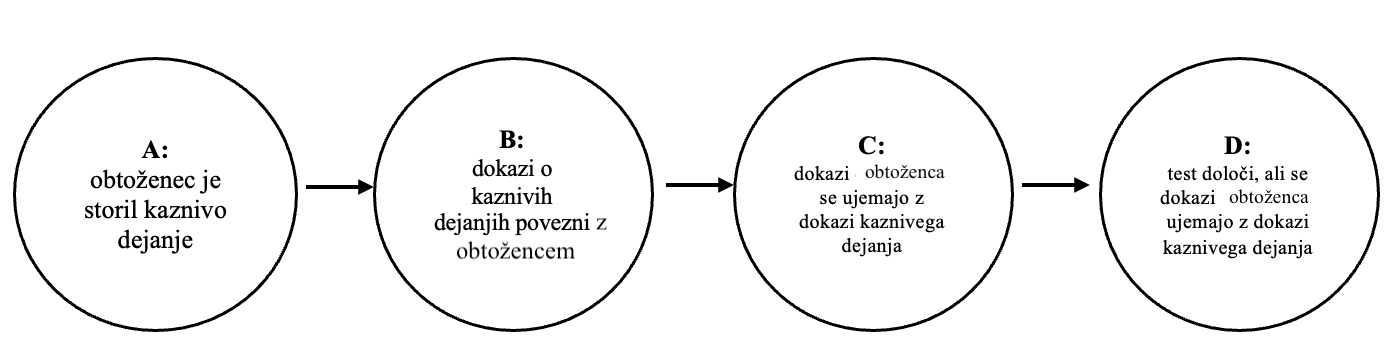
\includegraphics[scale=0.60]{slika_3.png}
    \caption{Vzorčna veriga dokazov}
 \end{figure}
 \\
\textit{Tožilčeva zmota}: pri tem enačimo  verjetnost, da oseba, ki ni vpletena v kaznivo dejanje, po naključju zagotovi dokaze, ki se ujemajo, 
tj. $P(C \lvert \neg B)$, s $P(\neg A \lvert C)$. Presega napako predhodne verjetnosti, saj si jo lahko 
predstavljamo kot dopolnitev te napake z dodatno napačno predpostavko $P(A) = P(B)$.\\\\
\textit{Napaka verjetnosti $P(\text{drugo ujemanje})$}: gre za zmoto, ko verjetnost, da oseba, ki ni vpletena v kaznivo dejanje, po 
naključju zagotovi dokaze, ki se ujemajo, tj. $P(C \lvert \neg B)$, enačimo z verjetnostjo
(imenujmo jo $q$), da ima vsaj en nedolžen član populacije ustreza dokazom. Posledica te napake je običajno močno pretiravanje z vrednostjo
dokaza $C$.\\\\
\textit{Zanemarjanje predhodnih verjetnosti}: to pomeni preprosto neupoštevanje predhodnih vrednosti, kot sta $P(A)$ in $P(B)$. Na splošno
se za zmoto zanemarjanja osnovne stopnje šteje, kadar je verjetnost dogodka podcenjena, ker dogodek ni tako nenavaden, kot se zdi,
ali precenjena, ker je dogodek bolj nenavaden, kot se zdi.\\\\
\textit{Napaka pri številčnem preračunavanju}: pri tem gre za zamenjavo verjetnost, da oseba, ki ni vpletena v kaznivo dejanje, po naključju 
zagotovi dokaze, ki se ujemajo, tj. $P(C \lvert \neg B)$ s pričakovanim številom drugih oseb,
ki bi jih bilo treba testirati, preden bi našli ujemanje. Ta zmota prav tako pretirava z vrednostjo dokaza $C$.\\\\
\textit{Pričakovane vrednosti, ki pomenijo edinstvenost}: če je velikost populacije približno enaka $1/P(\neg B \lvert C)$, potem mora biti
obdolženec edini primerek. \\\\
\textit{Zmota obrambnega odvetnika}: to se zgodi, ko se dokaz $C$ šteje za nepomembnega, ker visoka predhodna verjetnost $P(\neg A)$ (kar
se zgodi, če je na primer potencialno število osumljencev zelo veliko) še vedno povzroči visoko verjetnost $P(\neg B \lvert C)$. \\\\
\textit{Napaka baze podatkov obrambnega odvetnika}: za to napako gre, kadar verjetnost $P(\neg B \lvert C)$ temelji na drugačni populaciji,
kot jo določata verjetnosti $P(B)$ ali $P(A)$.\\\\
\textit{Zasliševalčeva zmota}: v tem primeru je dokaz neposredno priznanje krivde. Če to ni potrjeno, to pomeni, da uporabljamo verjetnost $P(D \lvert A)$ za
informiranje verjetnosti $P(A \lvert D)$. Napaka je, da ne upoštevamo $P(D \lvert \neg A)$. Če je $P(D \lvert A) \leq P(D \lvert \neg A)$, potem dokaz
nima vrednosti.\\\\
Poleg zmot, ki izhajajo iz osnovnega nerazumevanja pogojne verjetnosti, se druge zmote pojavijo zaradi neustreznega združevanja vpliva več dokazov:\\
\textit{Zmota odvisnih dokazov}: ta zmota, ki se včasih imenuje tudi dvojno štetje, se kaže v tem, da se dva ali več dokazov, ki so odvisni,
obravnava, kot da bi bili neodvisni, zaradi česar je izjava o njihovi skupni verjetnosti manjša, kot bi morala biti. Poseben primer te zmote je
\textit{logično odvisna dokazna zmota}, pri kateri en dokaz ni preprosto odvisen od drugega, ampak dejansko logično izhaja iz njega.\\\\
\textit{Napaka konjunkcije}: ta zmota se pojavi, kadar preiskovalec ne upošteva dejstva, da je dokaz sestavljen iz več kot enega negotovega dogodka,
in mu posledično pripiše večjo verjetnost, kot bi jo moral.

%%%%%%%%%%%%%%%%%%%%%%%%%%%%%%%%%%%%%%%%%%%%%%%%%%%%%%%%%%%%%%%%%%%%%%%%%%%%%%%%%%%%%%%%%%%%%%%%%%%%%%%%%%%%%%%%%%%%%%%%%%%%%%%%%%%%%%%%%%%%%%
%%%%%%%%%%%%%%%%%%%%%%%%%%%%%%%%%%%%%%%%%%%%%%%%%%%%%%%%%%%%%%%%%%%%%%%%%%%%%%%%%%%%%%%%%%%%%%%%%%%%%%%%%%%%%%%%%%%%%%%%%%%%%%%%%%%%%%%%%%%%%%
\subsection{Tožilčeva zmota}
Verjetnostno utemeljevanje pravnih dokazov se torej skrči na preprost vzročni scenarij: začnemo z neko hipotezo $H$ in opazujemo nek dokaz $E$.
Poznavanje pogojne verjetnosti $P(E \lvert H)$ nam omogoča, da spremenimo svoje prepričanje o verjetnosti $H$, če poznamo $E$. Veliko najpogostejših
napak v sklepanju izhaja iz osnovnega nerazumevanja pogojne verjetnosti. Še posebej pogost primer je zamenjava verjetnost dokaza $E$ glede na
hipotezo $H$ z verjetnost hipoteze $H$ glede na dokaze $E$ oziroma $P(E \lvert H)$ z $P(H \lvert E)$, torej ko napačno verjamemo, da je verjetnost 
naključnega znanstvenega ujemanja enaka verjetnosti, da je obtoženec nedolžen. To se pogosto imenuje napaka prenesenega pogojnika oziroma tudi 
tožilčeva zmota.\\\\
Tožilčeva zmota se pogosto pojavlja v kazenskem pravu, vendar jo pogosto ne prepoznajo, deloma zato, ker preiskovalci
nimajo močne intuicije o tem, kaj zmota sploh pomeni. Tožilčeva zmota je dobro znana statistična zmota, ki izhaja iz napačnega razumevanja
pogojnih verjetnosti in vprašanj večkratnega testiranja. Napaka temelji na predpostavki, da je $P(H \lvert E) = P(E \lvert H)$, pri čemer $H$
predstavlja primer, da se najdejo dokazi o obtožencu, $E$ pa primer, da je obtoženec nedolžen. Vendar ta enakost ne drži: čeprav je $P(H \lvert E)$
običajno zelo majhen, je lahko $P(E \lvert H)$ še vedno veliko večji. \\\\
Za lažjo predstavo si oglejmo primer. Naj se kri obtoženca ujema s krvjo storilca kaznivega dejanja. Ta krvna skupina je tako redka, 
da je verjetnost, da jo ima nekdo, le 1 proti 1000. Če si to statistiko razlagate tako, da obstaja le 1 proti 1000 možnosti, da je obtoženec 
nedolžen, ste žrtev tožilske zmote. Verjetnost naključnega ujemanja (pogostost krvnega profila) ste napačno združili z verjetnostjo vira (verjetnost, 
da je vir krvi nekdo drug kot obtoženec). V mestu z milijon prebivalci bi bilo približno 1000 ljudi z redkim krvnim profilom. Čeprav je torej 
res, da obstaja le verjetnost 1 proti 1000, da se kri naključne osebe ujema s krvjo zločinca, je verjetnost, da je oseba, ki ustreza redkemu 
profilu krvi, nedolžna, in sicer izključno na podlagi ujemanja dokazov, dejansko 999 proti 1000. \\\\
Do tožilčeve zmote lahko pride zaradi večkratnega testiranja, na primer pri primerjanju dokazov z veliko podatkovno bazo. Velikost podatkovne
zbirke povečuje verjetnost, da bo ujemanje ugotovljeno zgolj po naključju. \\\\
Če je $E$ dokaz in $H$ trditev,  da je obtoženi nedolžen, upoštevamo pogojne verjetnosti: \\
$P(E \lvert H)$ \dots verjetnost resničnosti dokaz $E$, kljub temu da je obtoženi nedolžen; \\
$P(H \lvert E)$ \dots verjetnost, da je obtoženi nedolžen kljub dokazu $E$. \\
Pri forenzičnih dokazih je ponavadi verjetnost $P(E \lvert H)$ majhna. Tožilec pa potem velikokrat sklepa, da je tudi verjetnost
$P(H \lvert E)$ majhna.
%(tožilstvo Lucie de Berk je na primer obtoženo ravno te napake)
Zgoraj napisani pogojni verjetnosti pa sta precej različni; uporabimo Bayesovo pravilo:
\[
   P(H \lvert E) = P(E \lvert H) \times \frac{P(H)}{P(E)}, \vspace{2mm}
\]
kjer je $P(H)$ verjetnost nedolžnosti in $P(E)$ verjetnost dokaza. Enačba kaže, da majhna pogojna verjetnost $P(E \lvert H)$ ne pomeni majhne
pogojne verjetnosti $P(H \lvert E)$ v primeru velike verjetnosti nedolžnosti in majhne verjetnosti dokaza. \\
Po Bayesovem pravilu je
\[
   P(E)=P(E \lvert H)P(H) + P(E \lvert \neg H)\times[1 - P(H)] \vspace{2mm}
\]
kjer je $P(E \lvert \neg H)$ verjetnost, da bodo dokazi identificirali krivega osumljenca; običajno je ta verjetnost blizu 1.

%%%%%%%%%%%%%%%%%%%%%%%%%%%%%%%%%%%%%%%%%%%%%%%%%%%%%%%%%%%%%%%%%%%%%%%%%%%%%%%%%%%%%%%%%%%%%%%%%%%%%%%%%%%%%%%%%%%%%%%%%%%%%%%%%%%%%%%%%%%%%%
\subsubsection{Primer - Tožilčeva zmota}
Za še boljšo predstavo zmote sledi predstavitev zmote na bolj kompleksnem primeru.\\\\
Slika 2 prikazuje populacijo 100 moških, starih 50 let, ki se ne zdravijo zaradi hipertenzije in imajo skupni holesterol 235 mg/dl in krvni tlak 120 mmHg. Pričakuje
se, da bo 9\% teh moških (predstavljeno z devetimi črtastimi kvadrati) čez 10 let imelo miokardni infarkt(MI). Ena četrtina moških je kadilcev (predstavljeno s 25
sivimi kvadrati); približno 16\% naj bi doživelo MI v 10 letih; zato bo $\frac{4}{25}$ kadilcev imelo MI (predstavljeno s črtastimi in sivimi kvadrati). \\
Število kadilcev, ki imajo MI, je očitno enako številu ljudi, ki imajo MI in so kadilci. Toda ali je delež kadilcev, ki imajo MI, enak deležu ljudi z MI, ki so kadilci? Iz
slike 2 je odgovor očitno ne; verjetnost, da ste kadilec glede na to, da ste imeli MI, torej:
\[
   P(\text{MI} \lvert \text{kadilec}) \ne P(\text{kadilec} \lvert \text{MI}), \vspace{2mm}
\]
ker
\[
   P(\text{MI} \lvert \text{kadilec}) = P(\text{črtasto} \lvert \text{sivo}) = \frac{4}{25} = 0,16 \vspace{2mm}
\]
in
\[
   P(\text{kadilec} \lvert \text{MI}) = P(\text{sivo} \lvert \text{črtasto}) = \frac{4}{9} = 0,44. \vspace{2mm}
\]
Vizualno opazimo, da delež sivih kvadratov, ki se prekrivajo s črtastimi kvadrati, ni enak deležu črtastih kvadratov, ki se prekrivajo s sivimi kvadrati.
\begin{figure}[!ht]\label{fig:slika1}
   \centering
   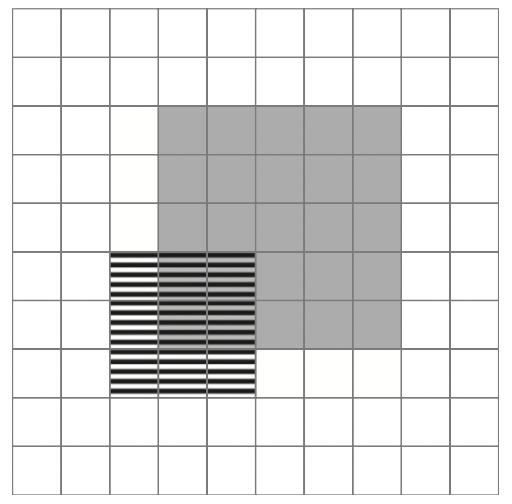
\includegraphics[scale=0.45]{slika1.png}
   \caption{Populacija, predstavljena s 100 kvadrati, z 9 črtastimi, 25 sivimi in 4 črtastimi in sivimi.}\vspace{2mm}
\end{figure}\\
Slika 3 prikazuje izjeme pri tožilčevi zmoti, predstavljeni na sliki 1. Sedaj imamo 16 črtastih kvadratov, 16 sivih in 4 pikčaste in sive kvadrate, ker je splošna
razširjenost črtastih in sivih kvadratov enaka, je
\[
   P(\text{črtasto} \lvert \text{sivo}) = P(\text{sivo} \lvert \text{črtasto}). \vspace{2mm}
\]
Tudi
\[
   P(\text{črtasto} \lvert \text{pikčasto}) = P(\text{pikčasto} \lvert \text{črtasto}), \vspace{2mm}
\]
saj sta obe verjetnosti enaki $0$. Oboje(podobno velike populacija in populacije brez prekrivanja) je ozka izjema zmote. \\
Po drugi strani pa so črtkani kvadrati na sliki 2 v celoti zajeti v sivih kvadratih; tako je
\[
   P(\text{sivo} \lvert \text{črtkano}) = 1, \quad \text{medtem ko je} \quad P(\text{črtkano} \lvert \text{sivo}) = 0,25. \vspace{2mm}
\]
Tožilčeva zmota velja, kadar je ena skupina podmnožica druge. 
\begin{figure}[!ht]\label{fig:slika2}
   \centering
   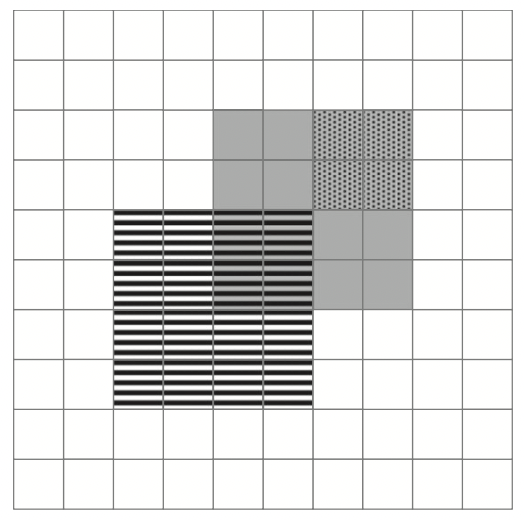
\includegraphics[scale=0.45]{slika2.png}
   \caption{Populacija, predstavljena s 100 kvadrati, z 16 črtastimi, 16 sivimi in 4 pikčastimi in sivimi.}\vspace{2mm}
\end{figure}

%%%%%%%%%%%%%%%%%%%%%%%%%%%%%%%%%%%%%%%%%%%%%%%%%%%%%%%%%%%%%%%%%%%%%%%%%%%%%%%%%%%%%%%%%%%%%%%%%%%%%%%%%%%%%%%%%%%%%%%%%%%%%%%%%%%%%%%%%%%%%%
%%%%%%%%%%%%%%%%%%%%%%%%%%%%%%%%%%%%%%%%%%%%%%%%%%%%%%%%%%%%%%%%%%%%%%%%%%%%%%%%%%%%%%%%%%%%%%%%%%%%%%%%%%%%%%%%%%%%%%%%%%%%%%%%%%%%%%%%%%%%%%
\section{Načini za izogib zmotam}
V zadnjih letih je statistika in verjetnost v kazenskem pravu napredovala. Sodniki, tožilstvo in porota se zavedajo nerazumevanja te znanosti, zato 
je statistika čedalje bolj vpletena že v učne programe pravnih fakultet, kar pripomore k boljšemu razumevanju statističnih analiz. Kljub temu so seveda 
zmote še vedno prisotne. V začetku dela sem omenila, da je razlaga statistične analize odvisna od vprašanj odvetnika, pri čemer veliko za izboljšanje 
ne moremo storiti. Poleg tega morajo biti statistični oziroma forenzični znanstveniki previdni z razlago, kajti ne smejo poseči v poroto. Torej kako 
se dejansko izognimo zmotam in s tem ne posežemo v pravna pravila na sodiščih in sodnih procesih.

%%%%%%%%%%%%%%%%%%%%%%%%%%%%%%%%%%%%%%%%%%%%%%%%%%%%%%%%%%%%%%%%%%%%%%%%%%%%%%%%%%%%%%%%%%%%%%%%%%%%%%%%%%%%%%%%%%%%%%%%%%%%%%%%%%%%%%%%%%%%%%
\subsection{Izogib zmotam z uporabo razmerja verjetnosti}
Vsem zgoraj opisanim zmotam je skupno to, da je resnična koristnost dokaza predstavljena na zavajajoč način - bodisi je pretirana bodisi podcenjena.
Prednost uporabe razmerja verjetnosti je, da odpravlja ugovor Bayesovemu izreku, in sicer upoštevanje predhodne verjetnosti za hipotezo,
kot je »kriv«. V veliki meri pomiri pomisleke pravnikov, ki bi sicer zavrnili Bayesov argument z utemeljitvijo, da je nedopustno predpostavljati 
predhodne verjetnosti o krivdi ali nedolžnosti.\\\\
Čeprav je uporaba razmerja verjetnosti kot sredstva za izogibanje zmotam in merjenje uporabnosti dokazov močno podprta, sem vseeno mnenja, da
imajo, po prebiranju različnih sodnih poročil, pravniki in laiki pogosto podobne težave pri razumevanju razmerja verjetnosti kot pri razumevanju
Bayesove teorije.

%%%%%%%%%%%%%%%%%%%%%%%%%%%%%%%%%%%%%%%%%%%%%%%%%%%%%%%%%%%%%%%%%%%%%%%%%%%%%%%%%%%%%%%%%%%%%%%%%%%%%%%%%%%%%%%%%%%%%%%%%%%%%%%%%%%%%%%%%%%%%%
\subsection{Učinkovitost Bayesove teorije pri zmanjšanju zmote obrambnega odvetnika}
Zmota odvetnika je manj znana različica pogostejše tožilske zmote. Pri zmoti odvetnika je porota spodbujena, da asociativnih dokazov ne upošteva 
kot nepomembnih, ne glede na to, kako redka je značilnost ujemanja.\\\\
Za ponazoritev si predstavljajte sojenje z enakim ujemanjem krvi kot pri tožilčevi zmoti, vendar z dodatnimi dokazi proti obtožencu, kot sta 
očividec in posedovanje orodja za kaznivo dejanje. Zagovornik lahko kljub temu poroti pove, da je verjetnost obtoženčeve krivde le 1 proti 1000. 
To bi bilo sicer pravilno, če bi obtožnica utemeljevala primer samo na podlagi ujemanja krvi, vendar obrambni odvetnik dejansko prosi poroto, 
naj ne upošteva drugih dokazov razen ujemanja krvi. To je zmota obrambnega odvetnika. Če obrambnemu odvetniku uspe prepričati poroto, da verjame 
tej napačni logiki, lahko dodatni dokazi o ujemanju krvi napačno zmanjšajo verjetnost krivde pri poroti.\\\\
Čeprav so učinki tožilčeve zmote lahko hujši kot učinki zmote odvetnika (krivična obsodba v primerjavi s krivično oprostitvijo), so porote morda 
bolj dovzetne za slednjo kot za prvo.

%%%%%%%%%%%%%%%%%%%%%%%%%%%%%%%%%%%%%%%%%%%%%%%%%%%%%%%%%%%%%%%%%%%%%%%%%%%%%%%%%%%%%%%%%%%%%%%%%%%%%%%%%%%%%%%%%%%%%%%%%%%%%%%%%%%%%%%%%%%%%%
\subsection{Učinkovitost Bayesove teorije pri zmanjšanju zasliševalčeve zmote}
To zmoto opredeljujemo kot zmoto, ki se kaže v tem, da izpovedni dokazi nikoli ne morejo zmanjšati verjetnosti krivde - v določenih okoliščinah 
lahko priznanje zmanjšal verjetnost krivde. Vprašanje je, kdaj natančno je priznanje znak krivde in kdaj ne. Priznanje poveča verjetnost krivde 
le, kadar je verjetnost priznanja, če je oseba kriva, večja od verjetnosti priznanja, če je oseba nedolžna. Če se $H$ nanaša na trditev, da je 
oseba kriva, $E$ pa na trditev, da oseba prizna, velja
\[
    P(H \lvert E) > P(H \lvert \neg E)
\]  
velja le pod pogojem, da je 
\[
    P(E \lvert H) > P(E \lvert \neg H).
\] 
\begin{trditev}
    Obstoj priznanja poveča verjetnost krivde, če in samo če je manj verjetno, da bo nedolžna oseba priznala kot kriva.
\end{trditev}
Slednjo trditev je mogoče izpeljati s pomočjo Bayesove teorije:
\begin{equation}\label{eq:btrditev}
    \frac{P(H \lvert E)}{P(\neg H \lvert E)} = \frac{P(H)}{P(\neg H)}  \times \frac{P(E \lvert H)}{P(E \lvert \neg H)}
\end{equation}
Na levi strani je 
\[
    \frac{P(H \lvert E)}{P(\neg H \lvert E)},
\] 
razmerje posteriornih verjetnosti krivde in nedolžnosti (tj. verjetnosti po 
upoštevanju priznanja). Enak je zmnožku dveh drugih razmerij na desni strani. Razmerje 
\[
    \frac{P(H)}{P(\neg H)}
\]
predstavlja razmerje predhodnih 
verjetnosti krivde in nedolžnosti (to je verjetnosti krivde in nedolžnosti pred upoštevanjem dejstva priznanja). Zadnje razmerje, 
\[
    \frac{P(E \lvert H)}{P(E \lvert \neg H)},
\] 
se imenuje razmerje verjetnosti in določa, kakšen vpliv bo imel nov dokaz (priznanje) na 
verjetnosti krivde in nedolžnosti. Posteriorna verjetnost krivde bo večja od predhodne verjetnosti krivde le, če bo razmerje verjetnosti 
večje od 1. Če pa je razmerje verjetnosti 
\[
    \frac{P(E \lvert H)}{P(E \lvert \neg H)} < 1,
\] 
priznanje dejansko postane kazalnik nedolžnosti. \\\\
Ni nujno, da iz vsega tega sledi, da bi bil obstoj priznanja v tej situaciji dokaz proti krivdi. V nasprotju s tem, bi lahko priznanje še vedno 
povečalo verjetnost krivde, tudi če je bolj verjetno, da bo nedolžna oseba priznala kot kriva. Takšna zamisel se zdi logično nemogoča, če 
pogledamo \eqref{eq:btrditev}. Vendar želim povedati, da enačba \eqref{eq:btrditev} morda ni prava formula za uporabo v tem primeru. Morda obstaja še eno empirično dejstvo, 
ki je pomembno za verjetnost krivde. V tem primeru bi morali uporabiti bolj zapleteno formulo, ki bi vključevala to dejstvo. Ker tu preučujemo 
dokazni učinek priznanja, ki je rezultat zaslišanja, verjetnost, ki jo iščemo, v resnici ni verjetnost, da je oseba X kriva, če je priznala, 
ampak verjetnost, da je oseba X kriva, če je priznala in če je bila zaslišana. Zato je treba razmerje posteriornih verjetnosti izraziti na 
naslednji bolj celovit način, pri čemer $I$ predstavlja trditev \textit{je bil zaslišan}:
\begin{equation}\label{eq:posteriorne}
    \frac{P(H \lvert E, I)}{P(\neg H \lvert E, I)} = \frac{P(H \lvert I)}{P(\neg H \lvert I)}  \times \frac{P(E \lvert H, I)}{P(E \lvert \neg H, I)}
\end{equation}
in z nadaljnjo razširitvijo prvega razmerja verjetnosti na desni strani \eqref{eq:posteriorne}
\begin{equation}\label{eq:razširitev}
    \frac{P(H \lvert E, I)}{P(\neg H \lvert E, I)} = \frac{P(H)}{P(\neg H)} \times \frac{P(I \lvert H)}{P(I \lvert \neg H)}  \times \frac{P(E \lvert H, I)}{P(E \lvert \neg H, I)}
\end{equation}
Da bi videli, zakaj je prvo razmerje na desni strani \eqref{eq:posteriorne} enakovredno produktu prvih dveh razmerij na desni strani \eqref{eq:razširitev}, najprej upoštevajmo naslednji dve osnovni verjetnostni resnici:
\begin{equation}\label{eq:ver1}
    P(H \lvert I) = \frac{P(H) \times P(I \lvert H)}{P(I)},
\end{equation}
\begin{equation}\label{eq:ver2}
    P(\neg H \lvert I) = \frac{P(\neg H) \times P(I \lvert \neg H)}{P(I)}.
\end{equation}
Če zdaj \eqref{eq:ver1} delim z \eqref{eq:ver2} dobim
\begin{equation}\label{eq:enakovredno}
    \frac{P(H \lvert I)}{P(\neg H \lvert I)} = \frac{P(H)}{P(\neg H)}  \times \frac{P(I \lvert H)}{P(I \lvert \neg H)}.
\end{equation}
Enačba \eqref{eq:enakovredno} dokazuje, da sta \eqref{eq:posteriorne} in \eqref{eq:razširitev} enakovredni.\\\\
Primerjajmo enačbo \eqref{eq:btrditev} z enačbo \eqref{eq:razširitev}, ki daje popolnejšo sliko stanja. Na levi strani je v vsakem primeru razmerje posteriornih verjetnosti krivde in nedolžnosti, s to 
razliko, da so v \eqref{eq:btrditev} te verjetnosti pogojene samo s priznanjem, medtem ko so v \eqref{eq:razširitev} pogojene tako s priznanjem kot z zaslišanjem. Prvo razmerje na desni strani je enako 
tako v \eqref{eq:btrditev} kot \eqref{eq:razširitev}: razmerje predhodnih verjetnosti $H$ in $\neg H$. Tudi zadnje razmerje na desni strani je v obeh primerih podobno: verjetnost priznanja glede na 
krivdo (in zaslišanje), deljena z verjetnostjo priznanja glede na nedolžnost (in zaslišanje). V enačbi \eqref{eq:razširitev} imamo na desni strani razmerje 
\[\frac{P(I \lvert H)}{P(I \lvert \neg H)},\] kar je verjetnost, da vas bo policija zaslišala, če je oseba kriva, deljena z verjetnostjo, da vas bo policija 
zaslišala, če je oseba nedolžna. To razmerje je večje od 1. Razumno je namreč pričakovati, da bo policija z večjo verjetnostjo izbrala za zaslišanje nekoga, 
ki je kriv, kot nekoga, ki je nedolžen. Prav to razmerje v \eqref{eq:razširitev} razkriva, kaj je narobe z zgornjo trditvijo, da se lahko verjetnost krivde po priznanju poveča le, 
če je $P(E \lvert H) > P(E \lvert \neg H)$. \\
To lahko pokažemo s preprostim proti primerom. Sprejmimo domnevo, da kriminalci pod policijskim nadzorom redkeje priznajo kot nedolžni ljudje. Recimo, da prizna 
le 40 odstotkov krivcev, medtem ko prizna 60 odstotkov nedolžnih. Ker je zaradi tega verjetnost priznanja glede na krivdo manjša od verjetnosti priznanja glede 
na nedolžnost, se zdi, da sledi, da zdaj obstoj priznanja ne more povečati verjetnosti krivde od tiste, ki je bila pred priznanjem. Toda predpostavimo še, 
da je verjetnost, da bo policija zaslišala krivega, devetkrat večja kot verjetnost, da bo zaslišala nedolžnega posameznika. Nazadnje predpostavimo, da je 
predhodna verjetnost, da je oseba X kriva, na podlagi vseh dokazov pred priznanjem, 0,75. \\
Verjetnosti, ki veljajo za opisano situacijo:\\ \vspace{2mm}
\[P(E \lvert H, I)  = 0,4  \]
\[P(E \lvert \neg H, I) = 0,6  \]
\[P(H) = 0,75  \]
\[P(\neg H) = 0.25  \]
\[\frac{P(I \lvert H)}{P(I \lvert \neg H)} = 9. \]


Sledi po enačbi \eqref{eq:razširitev}
\begin{equation}\label{eq:rezultat}
    \frac{P(H \lvert E, I)}{P(\neg H \lvert E, I)}  = \frac{P(H \lvert I)}{P(\neg H \lvert I)}  \times \frac{P(E \lvert H, I)}{P(E \lvert \neg H, I)} = \frac{0,75}{0,25} \times 9 \times \frac{0,4}{0,6} = 18
\end{equation}
Enačba \eqref{eq:rezultat} nam pove, da je verjetnost, da je oseba X kriva, ob upoštevanju vseh okoliščin, 18-krat večja od verjetnosti, da je nedolžna. Ker mora biti 
bodisi kriva bodisi nedolžna, lahko to razmerje uporabimo za pridobitev posteriorne verjetnosti krivde osebe X. Verjetnost, da je kriva, glede na to, 
da je priznala (in da je bil zaslišana), je 18/19 ali 0,95. Pred priznanjem je bila verjetnost krivde 0,75. Po priznanju se verjetnost krivde poveča 
na 0,95 kljub temu, da je verjetnost, da bo priznala, če je kriva, manjša od verjetnosti, da bo priznala, če je nedolžna. \\
S tem je dokaz, da je priznanje lahko dokaz krivde le, če je verjetnost priznanja glede na krivdo večja od verjetnosti priznanja glede na nedolžnost, popoln.

%%%%%%%%%%%%%%%%%%%%%%%%%%%%%%%%%%%%%%%%%%%%%%%%%%%%%%%%%%%%%%%%%%%%%%%%%%%%%%%%%%%%%%%%%%%%%%%%%%%%%%%%%%%%%%%%%%%%%%%%%%%%%%%%%%%%%%%%%%%%%%
%%%%%%%%%%%%%%%%%%%%%%%%%%%%%%%%%%%%%%%%%%%%%%%%%%%%%%%%%%%%%%%%%%%%%%%%%%%%%%%%%%%%%%%%%%%%%%%%%%%%%%%%%%%%%%%%%%%%%%%%%%%%%%%%%%%%%%%%%%%%%%
\section{Nadaljevanje sodnega procesa - medicinska sestra Lucia de Berg: Interpretacija verjetnosti na sodišču}
Sodišče je bilo mnenja, da verjetnostni izračun, ki ga je podal Henk Elfferson, pomeni, da je osumljenka vse dogodke, navedene v obtožnici, doživela naključno. Ti 
izračuni naj bi poseldično prikazovali, da je velika verjetnost, da obstaja povezava med izmeno osumljenke in pojavom incidenta. Te sklepi sodišča bi morali statistikom 
vzbujati dvome, saj se sodba dvoumna in lahko bi rekla, da je sodišče storilo znano tožilčevo zmoto. Po sklepu sodišča bi lahko rekli, da govorijo o verjetnosti, da se je nekaj zgodilo 
ob predpostavki, da je vse popolnoma naključno ali pa si sodbo sodišča razlagamo kot verjetnost, da se je nekaj naključno zgodilo. Te dve trditvi pa sta različni, kar lahko 
pokažem z naslednjimi formulami. Naj bo\\
$F$ \dots opazovani dogodek;\\
$H_0$ \dots trditev, da se dogodek zgodi naključno.\\
Henk Elffers je izračunal verjetnost $P(F \lvert H_0) < 342 \times 10^{-6}$, medtem ko je sodišče mislilo, da je Elffersonova izračunana  verjetnost v bistvu $P(H_0 \lvert F)$, 
kar pa je definicija tožilčeve zmote.\\\\
Torej poleg tega, da je bila uporabljena metoda za izračun verjetnosti nekoliko sporna, kljub kasnejšim popravkom, je na koncu prišlo še do napake na sodišču, zaradi 
nerazumevanja pogojnih verjetnosti. Če bi hoteli pravično sodbo, bi, po mojem mnenju, seveda morali najprej izbrati ustrezne metode za izračun vseh verjetnosti, predstavitev 
statistične analize na sodišču pa bi morala biti bolj temeljita in prilagojena razumevanju sodnikom, odvetnikom in poroti. Sodba se je kasneje ponovno odprla, 
zaradi ugovorov na uporabljene metode Henka Elffersona.\\\\
V tem kazenskem primeru lahko vidimo koliko je še pomanjkljivosti pri statistiki v kazenskem pravu. Težave ne nastopijo zgolj pri nerazumevanju 
verjetnostnih izračunov, ampak očitno je, da je včasih že z izbiro ustrezne metode veliko težav, kar lahko privede do napačnih zaključkov.

%%%%%%%%%%%%%%%%%%%%%%%%%%%%%%%%%%%%%%%%%%%%%%%%%%%%%%%%%%%%%%%%%%%%%%%%%%%%%%%%%%%%%%%%%%%%%%%%%%%%%%%%%%%%%%%%%%%%%%%%%%%%%%%%%%%%%%%%%%%%%%
\section{Izogibanje zmotam z uporabo Bayesovih \\omrežij}
Ker je največkrat težava v tem, da se večina odvetnikov in sodnikov ob pogledu na verjetnostne izračune in statistično analizo dokazov, ustraši, se mi 
zdijo Bayeosova omrežja dober predlog za predstavitev verjetnostnih izračunov.

%%%%%%%%%%%%%%%%%%%%%%%%%%%%%%%%%%%%%%%%%%%%%%%%%%%%%%%%%%%%%%%%%%%%%%%%%%%%%%%%%%%%%%%%%%%%%%%%%%%%%%%%%%%%%%%%%%%%%%%%%%%%%%%%%%%%%%%%%%%%%%
\subsection{Opredelitev}
Bayesova omrežja pomagajo določiti ustrezne verjetnostne formule, ne da bi prikazali njihovo polno algebrsko obliko, in omogočajo
skoraj popolno avtomatizacijo potrebnih verjetnostnih izračunov.
\begin{definicija}
   Bayesovo omrežje je verjetnostni grafični model, ki predstavlja množico spremenljivk in njihovih pogojnih odvisnosti prek usmerjenega
   acikličnega grafa.
\end{definicija}
Vozlišča teh usmerjenih acikličnih grafov predstavljajo spremenljivke (lahko so opazovane količine, latentne spremenljivke, neznani parametri
ali hipoteze). Povezave predstavljajo pogojne odvisnosti; vozlišča, ki niso povezana, predstavljajo spremenljivke, ki so pogojno neodvisne
druga od druge. Vsako vozlišče je povezano z verjetnostno funkcijo, ki kot vhodni podatek sprejme določen niz vrednosti za nadrejene spremenljivke
vozlišča in kot izhodni podatek poda verjetnost (ali verjetnostno porazdelitev, če je primerno) spremenljivke, ki jo predstavlja vozlišče. Puščice
predstavljajo razmerja pomembnosti, ki jih strokovnjak predvideva v okviru zadevnega problema sklepanja. Usmerjena povezava od vozlišča A do
vozlišča B pomeni, da ima A neposreden vpliv na B. Povezave med vozlišči se včasih razlagajo kot vzročne povezave, vendar opredelitev Bayesovih
omrežij ne zahteva, da povezave predstavljajo vzročni vpliv. Na splošno velja, da povezave v omrežju predstavljajo verjetnostna razmerja
pomembnosti. Značilnost Bayesovih omrežij je vključitev verjetnosti v obliki tabel, povezanih z vsakim vozliščem. To omogoča razlago narave in
moči odnosov med različnimi grafičnimi komponentami omrežja. Tabele verjetnosti vozlišč lahko torej obravnavamo kot sredstvo za povezovanje
modela s podatki.

%%%%%%%%%%%%%%%%%%%%%%%%%%%%%%%%%%%%%%%%%%%%%%%%%%%%%%%%%%%%%%%%%%%%%%%%%%%%%%%%%%%%%%%%%%%%%%%%%%%%%%%%%%%%%%%%%%%%%%%%%%%%%%%%%%%%%%%%%%%%%%
\subsection{Uporaba Bayesovih omrežij na sodišču}
Bayesova omrežja, ki temeljijo na Bayesovi teoriji in teoriji grafov, ponujajo forenzičnim znanstvenikom več prefinjenih možnosti. Tem metodam
se daje poseben poudarek, kadar je treba med konkurenčnimi hipotezami izbrati najverjetnejšo, izbira pa mora biti podprta z znanstveno utemeljeno
argumentacijo. Primerna so za analizo dogodka, ki se je zgodil, in napovedovanje verjetnosti, da je k temu prispeval katerikoli od več možnih
znanih vzrokov. Prednosti Bayesovih mrež se najbolj izrazito pokažejo na zapletenih področjih z več spremenljivkami. Kriminalistične aplikacije
Bayesovih omrežij segajo od prepoznavanja storilcev, posameznih in kompleksnih konfiguracij različnih vrst sledi ter problemov sklepanja, ki
vključujejo rezultate analiz DNK.\\
Ti grafični modeli verjetnosti bistveno izboljšajo vrednotenje verjetnostnih razmerij, ki se uporabljajo za ocenjevanje znanstvenih dokazov.
Omogočajo, da se lotimo kompleksnejših verjetnostnih analiz, kot bi bilo to mogoče s tradicionalnimi pristopi, kar še posebej pride prav pri primerih z ogromno dokazi. \\\\
Struktura Bayesovega omrežja v pravnem kontekstu je dovzetna za napačne predpostavke in napake v procesu ustvarjanja. Izbira vozlišč za dokaze je lahko
pristranska glede na to, kakšna vrsta argumenta je predstavljena. Argumenti obrambe ali tožilstva lahko na primer poudarjajo nasprotne sklepe
in zato vključujejo le podskupino dokazov. Če se za izdelavo ne uporablja dosleden okvir, lahko Bayesovo omrežje, ki jih oblikujejo različne stranke za en
primer, kažejo različne rezultate. Pri oblikovanju Bayesovega omrežja za pravno sklepanje ključnega pomena, da se oblikuje omrežje, ki je razumljivo poroti
in sodniku.\\\\
Prikaz Bayesovega omrežja se mora ujemati z intuitivnim pripisovanjem vzročno-posledičnih povezav med končno hipotezo, kot je »Obtoženec je kriv.«, podhipotezo
»Obtoženec je bil na kraju zločina.« in dokazi primera. Poleg težav, ki se pojavijo med postopkom strukturiranja, je problematično tudi sklepanje
iz omrežja, če se izvaja ob napačnih predpostavkah. Verjetnosti, tudi če temeljijo na strokovni presoji, so lahko pristranske zaradi dejavnikov
motenj v postopku pridobivanja podatkov. Metode za sklepanje morajo zato zagotoviti, da se verjetnosti omrežij ne razlagajo napačno kot dejstva in
da se izpostavi dejavnik negotovosti. Primerjati morajo verjetnosti za nasprotujoče si hipoteze in morajo zagotoviti okvir za pravnike, da iz
mreže sklepajo na argumente.

%%%%%%%%%%%%%%%%%%%%%%%%%%%%%%%%%%%%%%%%%%%%%%%%%%%%%%%%%%%%%%%%%%%%%%%%%%%%%%%%%%%%%%%%%%%%%%%%%%%%%%%%%%%%%%%%%%%%%%%%%%%%%%%%%%%%%%%%%%%%%%
%%%%%%%%%%%%%%%%%%%%%%%%%%%%%%%%%%%%%%%%%%%%%%%%%%%%%%%%%%%%%%%%%%%%%%%%%%%%%%%%%%%%%%%%%%%%%%%%%%%%%%%%%%%%%%%%%%%%%%%%%%%%%%%%%%%%%%%%%%%%%%
\section{Zaključek}
Statistika v kazenskem pravu je zelo razširjena veda, ki jo v prihodnosti čaka še veliko napredka. Njeni temelji se razlikujejo glede na države in pravno ureditev
tamkajšnjih sodišč. Zahteva pa tudi dobre temelje koncepta verjetnosti, statistični znanstvenik, ki se ukvarja z analizo in vrednotenjem dokazov, pa mora poznati
osnove prava.\\\\
V diplomski nalogi ugotovim, na podlagi pregleda nekaterih drugih metod, da je Bayesov pristop na splošno najboljši za vrednotenje dokazov, še posebaj v primeru,
ko se dokazi nanašajo na DNK ali laboratorijske analize. Koncept Bayesove metode je posodabljanje predhodnih oziroma apriornih verjetnosti začetnih hipotez in dokazov v
posteriorne s pomočjo razmerja  verjetnosti in Bayesovega pravila. Težava pristopa se pojavi pri določanju predhodnih verjetnosti, ker lahko različne metode za izračun
teh verjetnosti, dajejo na koncu različne rezultate. V delu pridem do ugotovitve, da je mogoče najbolje, da za določitev in izračun prehodnih verjetnosti poskrbijo
statistični znanstveniki, saj znajo v svoje modele vključevati tudi pravno teorijo. Težave pa nastanejo tudi pri vključevanju novih dokazov, ki so sodišču priloženi
tekom sodnega procesa in izključevanju nepomembnih oziroma nepotrebnih dokazov za sodni proces. Te dokaze vedno upoštevajo na drugačen način in jih drugače
vpeljejo oziroma izključijo iz svojih izračunov, kar bi v nekaterih primerih lahko bilo sporno. In ker se nekateri sodni procesi zaključijo na podlagi statistične
analize, bi po mojem mnenju tu morali biti malenkost bolj previdni in natančni. Torej do napačnih rezultatov lahko pridemo še pred predstavitvijo analize na sodišču, kar
je dobro prikazano tudi v primeru sodbe medicinski sestri Lucii de Berk, kjer je prišlo do problema, da je statistični znanstvenik na podlagi določenih podatkov
določil hipotezo, nato pa ta isti podatek uporabil za preverjanje te hipoteze. \\
Ko pa statistični znanstvenik predstavi analizo in rezultate na sodišču pa se lahko zgodijo tudi druge zmote. Podrobno sem opredelila Tožilčevo zmoto, ki je tudi
najpogostejša. Največkrat se verjetno zgodi, zaradi pomankljive predstavitve in razlage analize in, po mojih ugotovitvah, nezanimanja porote in sodnika, ko se predstavi
nek algebrski zapis izračuna. Zaradi zamenjave dveh različnih pogojnih verjetnosti, se zgodijo tudi napačni zaključki sodnih procesov. Zmotam, ki izhajajo iz napačnega
razumevanja pogojnih verjetnosti, se lahko izognemo z uporabo razmerja verjetnosti in Bayesove teorije, vendar sem prišla do sklepa, da je tudi pri tem razumevanju
formulacij in izračunov veliko težav. \\
Glavna ugotovitev dela je, da se lahko s pomočjo Bayesovih omrežij izognemo zmotam, saj ne prikažejo polno algebrsko obliko verjetnostne formule, omogočajo skoraj popolno
avtomatizacijo potrebnih verjetnostnih izračunov in več prefinjenih možnosti. Ponovno pa je pomembno, da se za izdelavo uporablja dosleden okvir, saj lahko Bayesovo omrežje,
ki jih oblikujejo različne stranke za en primer, kaž različne rezultate. Ker pa je v praksi ponavadi v sodni proces vključeno ogromno dokazov, ki jih težko analiziramo s
tradicionalnimi pristopi, nam pridejo Bayesova omrežja prav, saj omogočajo kompleksnejše analize.

%%%%%%%%%%%%%%%%%%%%%%%%%%%%%%%%%%%%%%%%%%%%%%%%%%%%%%%%%%%%%%%%%%%%%%%%%%%%%%%%%%%%%%%%%%%%%%%%%%%%%%%%%%%%%%%%%%%%%%%%%%%%%%%%%%%%%%%%%%%%%%
%%%%%%%%%%%%%%%%%%%%%%%%%%%%%%%%%%%%%%%%%%%%%%%%%%%%%%%%%%%%%%%%%%%%%%%%%%%%%%%%%%%%%%%%%%%%%%%%%%%%%%%%%%%%%%%%%%%%%%%%%%%%%%%%%%%%%%%%%%%%%%
%%%%%%%%%%%%%%%%%%%%%%%%%%%%%%%%%%%%%%%%%%%%%%%%%%%%%%%%%%%%%%%%%%%%%%%%%%%%%%%%%%%%%%%%%%%%%%%%%%%%%%%%%%%%%%%%%%%%%%%%%%%%%%%%%%%%%%%%%%%%%%

\end{document}
